\cleardoublepage

\chapter{Arquitectura e Implementación}
\label{ch:Capitulo4}

Existen múltiples niveles de implementación del prototipo planteado en este documento. El nivel más básico e imprescindible implica un ordenador con SO Linux que actuará como controlador de la infraestructura de dispositivos que dan forma al sistema en su conjunto, esto será referido en adelante como \gls{gateway}.


\section{Despliegue IoT de la solución domótica}
\label{ch:Capitulo4.1}
\vspace{1cm}

Para disponer de una base tecnológica sólida, pero fácil de adquirir, sobre la que experimentar y entender la complejidad de una suite domótica y sus planteamientos, en este proyecto se opta por usar hardware amigable como \verb|Raspberry Pi| para el \gls{gateway} y placas microcontroladoras \verb|nodeMCU| y las comúnmente llamados \verb|modulos ESP8266|, que disponen de una extensa comunidad de usuarios y documentación. En esa misma linea se buscará software libre. No sólo se puede aprovechar gran parte del trabajo ya creado en programación de \gls{script} para dispositivos como sensores y actuadores, aparte de ofrecer libertad para el usuario final de adaptar y modificar a su criterio tanto el software como el hardware. El \gls{gateway} actúa como concentrador de las conexiones de nodos, y dispone de los servicios necesarios para actuar como \verb|broker| de información para el servidor \verb|Node.js| que sera el núcleo del sistema, facilitando conexiones a clientes, los cuales mediante una \gls{app} móvil podrán conectarse para operar la solución domótica. En la siguiente figura~\ref{globalsystemdeployment} se observa como la aplicación móvil que se desarrollara, puede conectarse a través de la red de internet o de manera directa al router domestico, el conectara a su vez con el \gls{gateway} a través de una conexión de cable. El \gls{gateway} establece así el limite externo de la red de este despliegue de \gls{iot} y es a la vez el proveedor de servicios para la aplicación móvil, eliminado servicios de aplicación de terceros alojados en la red de internet para que pueda operar.

\begin{figure}[hbt!]
\label{globalsystemdeployment}
\centering
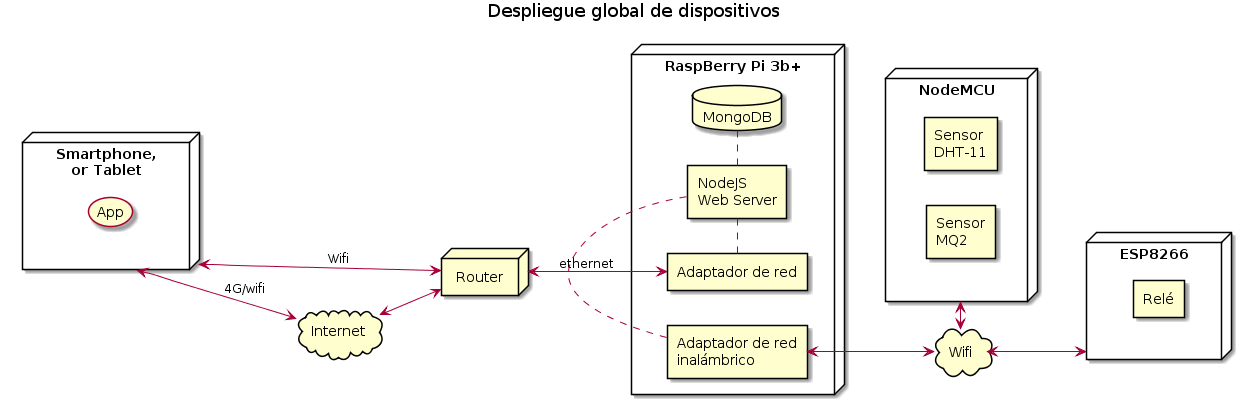
\includegraphics[height=2.2in]{figures/diagrams/physical-devices/global.png}
\caption[Diagrama de despiegue global de dispositivos]{Diagrama de despliegue global de dispositivos\footnotemark}
\end{figure}


\section{Definición del gateway}
\label{ch:Capitulo4.2}

El \gls{gateway} representa el núcleo de nuestra suite domótica. Al no existir una dependencia de procesos externos y computación en la red de internet, este elemento representa el dispositivo en la posición mas elevada de la jerarquía de la suite domótica. Los nodos dispuestos en un hogar lo usan como concentrador de comunicaciones para que el sistema opere, y la aplicación móvil lo usa como servidor para obtener la información registrada por esos dispositivos e interactuar con ellos. Si bien los nodos son capaces de registrar datos por su cuenta, estos deben ser entregados en el \gls{gateway} para ser procesados de forma útil para la aplicación.

\vspace{1cm}

La selección de \verb|Raspberry Pi| como plataforma de hardware se basa en dos características simples: es barato, de bajo consumo eléctrico e integra dos adaptadores de red. No está clasificado como \verb|Open Hardware| pero su proyecto goza de buena reputación en el mundo educativo y se considera una organización benéfica con el objetivo de acercar la electrónica a todo el mundo. Además, goza de una gran presencia en el mercado de electrónica, por lo cual es fácil de adquirir y ha acumulado una extensa comunidad de usuarios que muestran su uso mediante tutoriales y experimentos. Adicionalmente es de un reducido tamaño que permite ubicarlo con facilidad en lugares estrechos o difícilmente accesibles, además de su imperceptible ruido al operar. El modelo concreto para el desarrollo del \gls{gateway} es la \verb|Rapsberry Pi3b+| que dispone de capacidad de procesador y memoria RAM suficiente para operar todo el software necesario. Este modelo no integra un almacenamiento interno propio, pero la interfaz de la placa incluye una ranura de tarjetas micro-SD compatible con prácticamente todas las opciones de tamaño de almacenamiento disponibles en el mercado. Se precisan de al menos 4 \gls{gb} de espacio disponible en la memoria del sistema, y es recomendable exceder este mínimo siempre que sea posible, ya que la acumulación de datos con el paso del tiempo por parte del ordenador puede crecer indefinidamente.

\vspace{1cm}

El \gls{gateway} ejecuta \verb|Raspbian|. Un \gls{so} \verb|GNU/Linux| diseñado específicamente para la arquitectura ARMv7 de los distintos modelos de ordenadores Raspberry. Concretamente, en este proyecto se utiliza la serie de distribuciones \verb|Lite|, orientadas a la ejecución del sistema operativa mediante interfaz de linea de comandos en terminal. Esta decisión está fundamentada en desprenderse de la necesidad de periféricos externos e interfaces de \verb|I/O| analógicas para controlar el \gls{so}. Toda configuración del sistema será realizada mediante conexiones por \gls{ssh}. El proceso de instalación y configuración de conexiones esta ampliado en el apéndice~\ref{AppendiA:Key2} del documento. La selección de esta distribución en lugar de un \gls{so} estrictamente orientado a \gls{iot}, o para sistemas empotrados, se debe a la flexibilidad de aplicaciones y servicios que pueden instalarse durante los periodos de prueba y diseño.

\vspace{1cm}

Una vez establecidos los canales de comunicación, se instalarán aplicaciones que permitirán ejecutar los servicios necesarios para actuar como \gls{gateway}. La estrategia de comunicación entre los distintos dispositivos que conforman la suite domótica se basa en un servidor \verb|NodeJs| que establece conexiones vía \gls{wifi} de 2.4Gh con los nodos mediante el protocolo \gls{mqtt}. El servidor a su vez establece conexión con la aplicación móvil vía \gls{wifi} o internet, mediante el protocolo \gls{https}. Se realizara una descripción mas concisa del software necesario en el nodo principal en el apartado \ref{ch:Capitulo4.4}.


\section{Instalación y configuración del gateway}
\label{ch:Capitulo4.3}
 Utilizando los repositorios de distribuciones oficiales de \gls{so} de Raspberry Pi, se descarga e instala la versión \verb|lite| de \verb|Raspbian| en la tarjeta SD que se inserte en la \verb|Raspberry Pi|. Para establecer una conexión SSH por terminal es necesario crear un fichero con nombre \verb|ssh| en la raíz de la unidad de almacenamiento previamente al primer arranque del \gls{so}. La distribución originalmente estaba configurada por defecto con la conexión de \gls{ssh} abierta en el puerto 22, pudiendo acceder con el usuario \verb|pi| y la contraseña \verb|raspberry|. Este dato era ignorado por los usuarios menos experimentados y esto supuso una brecha de seguridad en todos las distribuciones que no fueron configuradas por los usuarios según las indicaciones de la propia \href{https://www.raspberrypi.org/documentation/configuration/security.md}{documentación de Raspberry}~\cite{securingyourraspberrypi}. En el primer arranque del SO de la Raspberry se establecerán las configuraciones básicas para las sucesivas conexiones \gls{ssh} basadas en autenticación con clave privada.
 
 \vspace{1cm}

 De las estrategias disponibles para esta configuración, se crearán las claves en el equipo remoto que se conectará al \gls{gateway}, entregando mediante la primera conexión \gls{ssh} con terminal la clave pública y almacenando la clave privada en el equipo remoto, reduciendo así el riesgo de ser expuesta fuera del dominio local del equipo. Para disponer de flexibilidad de conexión independientemente del \gls{so} del equipo remoto, la clave privada tendrá un formato \verb|OpenSSH|, fácil de incluir en \verb|Windows| o \verb|Linux| ya sea mediante conversión de la clave a formato \verb|PPK| o como fichero accesible para aplicaciones de desarrollo, transferencias de ficheros, y/o control de versiones que integran conexiones \gls{ssh} configurables (GitHub, Filezilla, Eclipse, etc). Los pasos necesarios para establecer conexiones cifradas robustas pueden encontrarse en el Anexo~\ref{AppendiA:Key2}.

\vspace{1cm}

Se establece la capacidad del \gls{gateway} para su adaptador de red \gls{wifi} de 2.4ghz, para actuar como punto de acceso~\cite{raspberrypiasaccesspoint} mediante un acceso vía usuario y contraseña, con \verb|WPA2| y gestión de claves \verb|WPA-PSK|. De esta forma, se despliega un punto de acceso de red inalámbrica que permitirá a otros dispositivos incorporarse a la suite domótica. En la figura~\ref{deploydevicesGateway} se observa una representación de despliegue de dispositivos donde los nodos, en diferentes plataformas de hardware y con distintos roles de actuadores o sensores, conectándose a la misma red inalámbrica generada por el adaptador de red \gls{wifi} integrado en el hardware del \gls{gateway}.

\begin{figure}[hbt!]
\label{deploydevicesGateway}
\centering
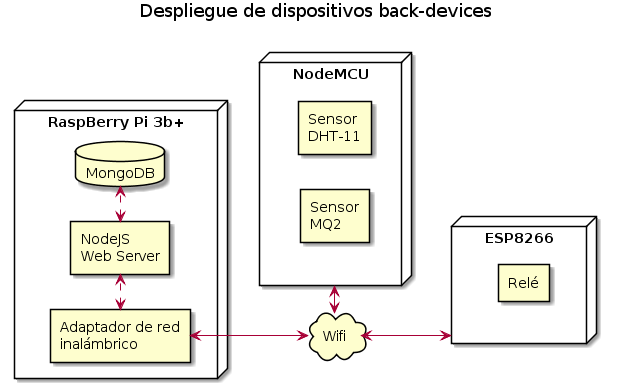
\includegraphics[height=2.5in]{figures/diagrams/physical-devices/back-devices.png}
\caption[Diagrama de despliegue de back-end]{Diagrama de despliegue de dispositivos y gateway\footnotemark}
\end{figure}

\vspace{1cm}

Las placas seleccionadas para actuar como nodos del sistema están basadas en el \gls{soc} \gls{wifi} \verb|ESP8266| y su firmware esta escrito en lenguaje \verb|LUA|, sin embargo, su código es habitualmente escrito en \verb|C| con un alto nivel mediante herramientas de desarrollo como \verb|Arduino IDE|. El proceso de subida de código en un lenguaje especifico que es transformado a otro lenguaje y subido a una placa microcontrontrolador cuyo lenguaje es distinto para sobreescribir el firmware se conoce como \verb|compilación cruzada|. Y permite una manera fácil de programar en alto nivel el código que hace funcionar una placa con \gls{soc} como las placas nodeMCU o los chips ESP8266. El código programado por el desarrollador se conoce en Arduino como \verb|sketch|. El proceso de subida de un \gls{sketch} a una placa mediante el entorno de desarrollo de Arduino se realiza mediante \gls{usb}. El proceso de instalación y configuración del entrono de desarrollo de Ardunio por linea de comandos, así como una primera prueba de funcionamiento del procedimiento esta detallado en el apendiceA\ref{AppendiA:Key2}. Es importante haber verificado el correcto funcionamiento de estas instrucciones antes de proseguir con el desarrollo.

\vspace{1cm}


Habiendo verificado el proceso de subida es necesario probar que la conexión inalámbrica y la comunicación mediante el protocolo \gls{mqtt} es correcta, con un código de prueba. El proceso es el mismo que en la etapa de pruebas: Instanciar un nuevo proyecto, incluir el código, subir el \gls{sketch} en la placa y probar la comunicación de la placa con el servidor. Es necesario además agregar las librerías necesarias, en el caso que ocupa este proyecto se utiliza la librería \verb|PubSubClient de Nick O'Leary|, un cliente ligero de \gls{mqtt} que posee buena estabilidad y fácil integración en desarrollo.

\begin{verbatim}
    cd ~/Arduino
    arduino-cli lib search PubSubClient
    arduino-cli lib install "PubSubClient"
    arduino-cli sketch new testmqtt
    nano test/testmqtt.ino
\end{verbatim}

El código de prueba de \gls{mqtt} incluye la librería de ESP8266WiFi.h que no es necesario añadir mediante el instalador de librerías, ya que este viene incluido en el core de tarjetas de terceros que se incluyo anteriormente para el chip esp8266. De esta forma, el código incluye los parámetros de conexión \gls{wifi} para el adaptador de red inalámbrico del nodo principal y la conexión al servicio de \gls{mqtt} así como la publicación de topics. El siguiente, es un ejemplo básico para hacer pruebas es una ligera modificación del ejemplo contenido en la ruta \path{~/Arduino/libraries/PubSubClient/examples/mqtt_basic/mqtt_basic.ino}.


\begin{verbatim}
#include <ESP8266WiFi.h>
#include <PubSubClient.h>

const char* ssid = "edomus";
const char* password = "sistemaguardian1970.";
const char* mqtt_server = "192.168.4.1";

WiFiClient espClient;
PubSubClient client(espClient);
char msg[50];
long lastMsg = 0;
int value = 0;

 
void setup_wifi() {
  delay(10);
  // We start by connecting to a WiFi network
  WiFi.begin(ssid, password);
  while (WiFi.status() != WL_CONNECTED) {
    delay(500);
  }
  randomSeed(micros());
}
 
void callback(char* topic, byte* payload, unsigned int length) {
  // Switch on the LED if an 1 was received as first character
  if ((char)payload[0] == '1') {
    digitalWrite(BUILTIN_LED, LOW); 
  } else {
    digitalWrite(BUILTIN_LED, HIGH);
  }
}
 
void reconnect() {
  // Loop until we're reconnected
  while (!client.connected()) {
    // Create a random client ID
    String clientId = "nodemcuClient-test";
    clientId += String(random(0xffff), HEX);
    
    // Attempt to connect
    if (client.connect(clientId.c_str())) {
      client.publish("outTopic", "hello world");
      client.subscribe("test");
    } else {
      delay(5000);
    }
  }
}

void setup() {
  pinMode(BUILTIN_LED, OUTPUT);
  setup_wifi();
  client.setServer(mqtt_server, 1883);
  client.setCallback(callback);
}
 
void loop() {
  if (!client.connected()) {
    reconnect();
  }
  client.loop();
  long now = millis();
  
  if (now - lastMsg > 2500) {
    lastMsg = now; 
    ++value;
    snprintf (msg, 50, "hello world #%ld", value);
    client.publish("test/msg", msg);
  }
}
\end{verbatim}

Una vez subido el sketch a la placa según los pasos anteriormente indicados, podemos realizar una llamada a la placa mediante el cliente de \gls{mqtt} instalado en el nodo principal. El cual generara una salida de texto sin fin. También se puede operar el led embebido en la placa con el argumento 0 o 1. Con esto, queda probado que el proceso de subida y la placa están en condiciones óptimas de funcionamiento.

\begin{verbatim}
    mosquitto_sub -h localhost -t test/msg
    mosquitto_pub -h localhost  -t test -m "1"
    mosquitto_pub -h localhost  -t test -m "0"
\end{verbatim}

\section{Scritps de generación de sckets para nodos}
\label{ch:Capitulo4.3.1}

Crear un \gls{sketch} mediante un script puede variar en su complejidad en el grado de cuantos argumentos reciba y que tan flexible se desea que sea su comportamiento. Sea cual sea el tipo de \gls{sketch} que se busque crear, se debe mantener una estructura de carga de librerías y constantes, un constructor y un bucle de ejecución. Considerando las necesidades del proyecto, se requiere que el script reciba los siguientes argumentos de entrada:

\begin{itemize}
  \item Modelo de la placa microcontroladora en la que se sube el \gls{sketch}.

  \item Modelo del sensor/actuador que va a conectarse en el GPIO de la placa microcontroladora.

  \item Valor numérico del pin de conexión de I/O en el que se conectara el sensor/actuador.
  
  \item Nombre de la estancia en la que se planea ubicar la placa microcontroladora.
\end{itemize}

Con esta estrategia, el administrador de la suite domótica puede añadir nuevos sensores y actuadores al abanico de opciones disponibles en la aplicación del usuario.

\subsection{Generador de sketch dinamicos para nodos}
l\label{ch:Capitulo4.3.2}

El objetivo ultimo del \gls{script} es generar un \gls{sketch} de Arduino que pueda compilarse y subirse a la placa correctamente, sin embargo, hasta que se reciben los argumentos solo es posible disponer de una plantilla genérica con secciones que deben ser rellenadas en base a las opciones que se indicaran en argumentos mas adelante. El modelo de plantilla básico puede constituirse con código previamente escrito en diferentes ficheros para luego ser ordenadamente ensamblados en un único fichero de código. En el caso de este proyecto, se crea una estructura de carpetas constituida por un directorio principal, el script generador, un directorio con las secciones de código común a todos los \gls{sketch} y directorios separados para cada sensor/actuador disponible en la aplicación. Para la prueba inicial incluiremos el código del sensor DHT11 para un configurar una placa detectora de temperatura y humedad. En términos generales, un sensor/actuador requiere de 4 bloques de código que integrar en código común, las librerías y constantes, la configuración inicial del setup, la resolución de callback que atiende peticiones concretas del servidor y el código del bucle que sera requerido por el protocolo \gls{mqtt} para publicar de manera constante. En la figura~\ref{sketchgeneratordiagram} se muestra como las diferentes secciones comunes a todos los códigos son combinadas con las secciones especificas de código en función de los argumentos definidos para el script.

\vspace{0.5cm}
\begin{figure}[hbt!]
\label{sketchgeneratordiagram}
\centering
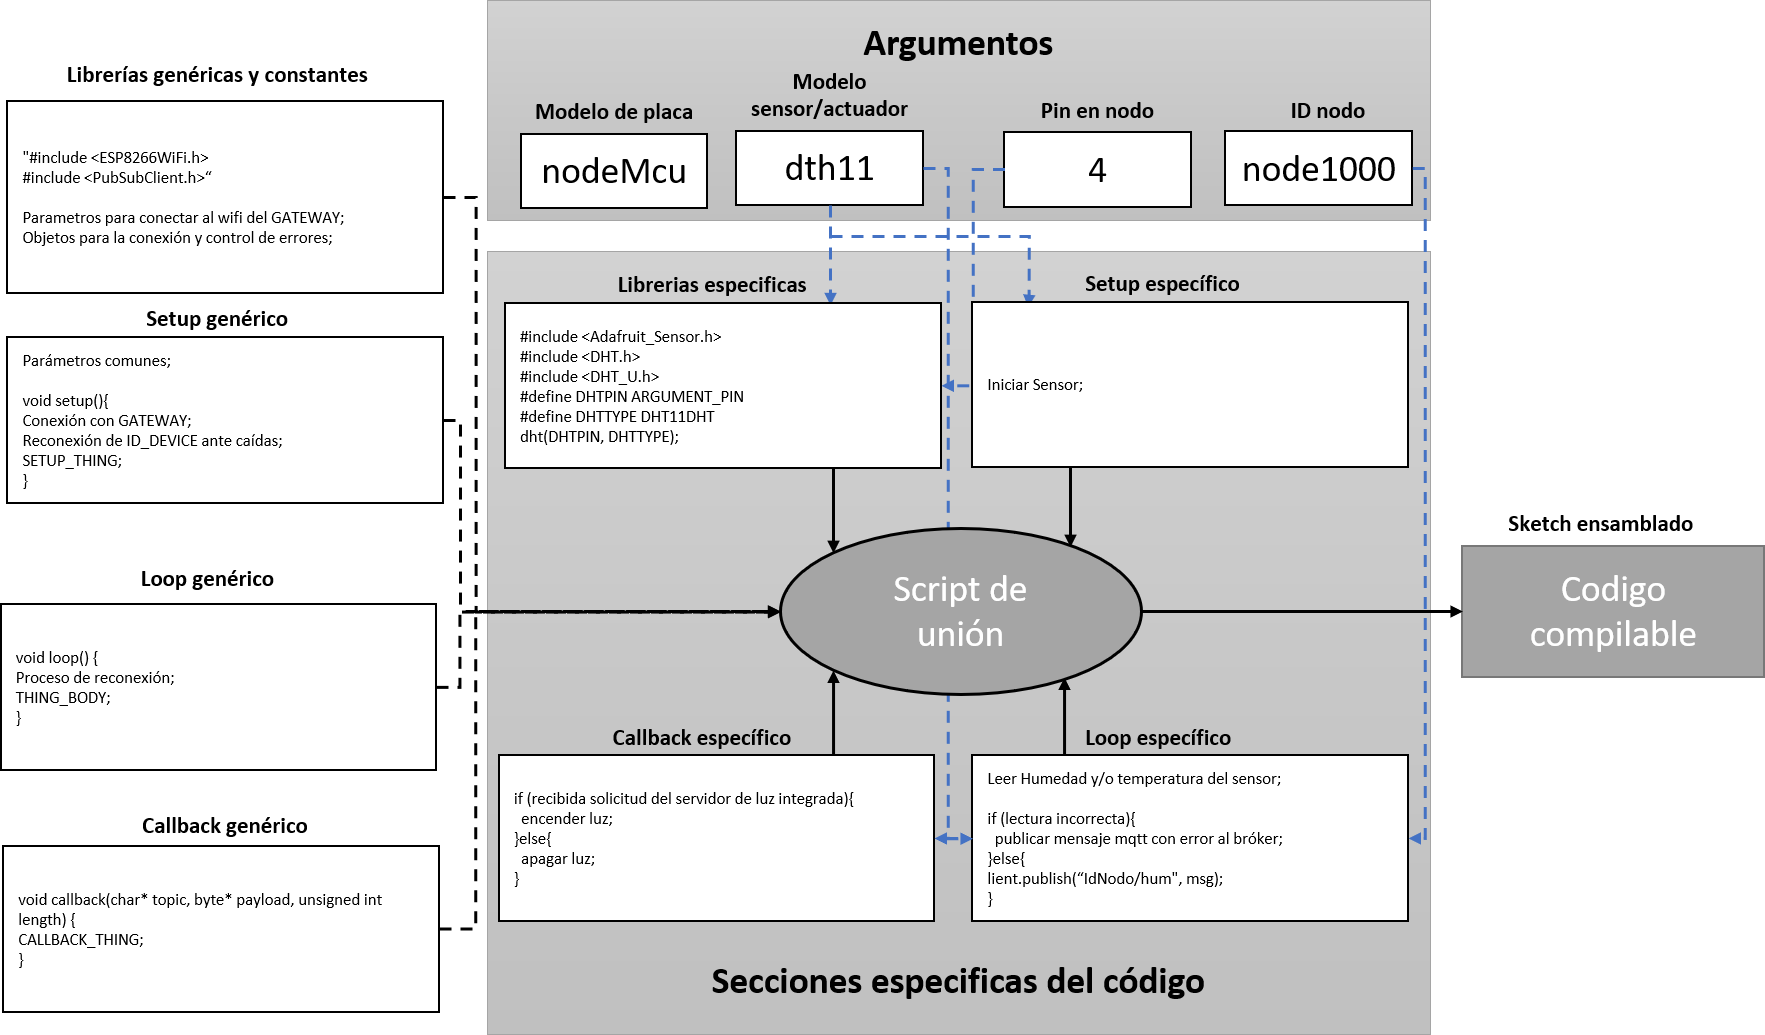
\includegraphics[height=2.6in]{figures/sketchgenerator.png}
\caption[Esquema de generación de sketch por partes]{Esquema de generación de sketch por partes\footnotemark}
\end{figure}

El proceso que debe preparase para que este esquema se cumpla requiere de la creación de directorios con los contenedores de codigos por partes que serannecesarios apra generar un \gls{sketch} valido que pueda compilarse y subirse a un nodo.

\begin{verbatim}
    cd ~
    mkdir sketchgenerator
    touch sketchgenerator/sketchgenerator
    mkdir sketchgenerator/general
    touch sketchgenerator/general/loop
    touch sketchgenerator/general/setup
    touch sketchgenerator/general/callback
    mkdir sketchgenerator/dht
    touch sketchgenerator/dht/dht11Lib
    touch sketchgenerator/dht/dht11Loop
    touch sketchgenerator/dht/dht11Setup
    touch sketchgenerator/dht/dht11Callback
\end{verbatim}

Con esta estructura, el \gls{script} tendrá que construir un fichero de extensión .ino válido en la ruta de destino necesaria para que posteriormente arduino-cli pueda compilarlo y subirlo a la placa microcontroladora conectada a un puerto \gls{usb} del nodo principal. Primero consideraremos el código de uso común a todos los \gls{sketch}.

\begin{verbatim}
    nano sketchgenerator/general/setup
\end{verbatim}

Considerando que el sensor DHT11 posee cierto código que se incluye en la función setup, se usara una cadena de caracteres a modo de centinela, el cual sera sustituido por el código definido en un fichero concreto (dht11Setup, en este caso) situado en el directorio del sensor definido por los argumentos del script generador. Dicho centinela en este código aparece como \verb|SETUP_THING|. Adicionalmente, en este segmento, y demás casos, se incluirá el centinela \verb|ID_DEVICE| que sera entregado en los argumentos del script para identificar una placa de manera inequívoca por parte del servidor.

\begin{verbatim}
long lastMsg = 0;
char msg[50];
int value = 0;

void setup() {
  pinMode(BUILTIN_LED, OUTPUT);
  setup_wifi();
  client.setServer(mqtt_server, 1883);
  client.setCallback(callback);

  SETUP_THING
}

void setup_wifi() {
  delay(10);
  WiFi.begin(ssid, password);
  while (WiFi.status() != WL_CONNECTED) {
    delay(500);
  }
}

void reconnect() {
  while (!client.connected()) {
    if (client.connect("ID_DEVICE")) {
      client.publish("ID_DEVICE/status", "hello world");
      client.subscribe("ID_DEVICE");
    } else {
      delay(5000);
    }
  }
}
\end{verbatim}

Para que el servidor pueda realizar peticiones concretas a una placa, está, debe resolver mediante la función callback los argumentos de entrada por \gls{mqtt} cuando se invoque un topic al que este suscrita dicha placa. En esta sección del código se incluye un centinela \verb|CALLBACK_THING| que sera sustituido por la lógica correspondiente a cada sensor/actuador. En general, esta sección de código esta planificada para ser usado por actuadores que pueden tener distintos estados, como un relé (encendido o apagado).

\begin{verbatim}
    nano sketchgenerator/general/callback
\end{verbatim}

\begin{verbatim}
void callback(char* topic, byte* payload, unsigned int length) {
  CALLBACK_THING
}
\end{verbatim}


El siguiente segmento de código común corresponde al bucle sin fin de un \gls{sketch}. Al igual que en el caso anterior, una sección del código deberá ser rellenada por las particularidades del sensor. Para este caso se ha definido un centinela \verb|MAIN_BODY|.

\begin{verbatim}
    nano sketchgenerator/general/loop
\end{verbatim}

\begin{verbatim}
void loop() {
if (!client.connected()) {
    reconnect();
  }
  client.loop();
  long now = millis();
  if (now - lastMsg > 2500) {
    lastMsg = now;
    MAIN_BODY
  }
}
\end{verbatim}

Para las secciones de código de un sensor como el DHT se requiere de las librerías, funciones auxiliares y constantes propias.
\begin{verbatim}
    nano sketchgenerator/dht/dht11Lib
\end{verbatim}

\begin{verbatim}
#include <Adafruit_Sensor.h>
#include <DHT.h>
#include <DHT_U.h>
#define DHTPIN ARGUMENT_PIN
#define DHTTYPE DHT11
DHT dht(DHTPIN, DHTTYPE);
\end{verbatim}

También es necesario el segmento de código que se incluye en la función setup.
\begin{verbatim}
    nano sketchgenerator/dht/dht11Setup
\end{verbatim}

\begin{verbatim}
dht.begin();
\end{verbatim}

La sección de callback de este sensor es limitada, ya que a la hora de atender peticiones expresas del servidor, como máximo se podría requerir las medidas del sensor, como añadido funcional, podemos manipular la luz integrada del sensor.

\begin{verbatim}
    nano sketchgenerator/dht/dht11Callback
\end{verbatim}

\begin{verbatim}
if ((char)payload[0] == '1')
{
    digitalWrite(BUILTIN_LED, LOW);
}
else
{
    digitalWrite(BUILTIN_LED, HIGH);
}
\end{verbatim}

Y por ultimo el segmento de código que sera invocado en la función loop que incluye la respuesta del cliente \gls{mqtt}. Este segmento de código también incluye centinelas que deben ser sustituidos en base a los argumentos del generador de \gls{sketch}, ya que de otra forma no seria posible definir los topics a los que responderá la placa cuando el nodo solicite información.
\begin{verbatim}
    nano sketchgenerator/dht/dht11Loop
\end{verbatim}

\begin{verbatim}
float h = dht.readHumidity();
float t = dht.readTemperature();
if (isnan(h) || isnan(t))
{
    snprintf (msg, 75, "{'status':'error', 'message':'Error in DHT11 sensor'}", value);
    client.publish("nodemcudht11", msg);
}
else
{
    snprintf (msg, 75, "'%f'", t);
    client.publish("TOPIC_PLACA/temp", msg);
    snprintf (msg, 75, "'%f'", h);
    client.publish("TOPIC_PLACA/hum", msg);
}
\end{verbatim}

Con todo este código por segmentado puede constituirse un \gls{sketch} valido siempre que se encadene en el orden correcto con las sustituciones adecuadas. El script se ejecutara en el entorno de \verb|Bash|, y realizara la recepción de los argumentos, validación de los mismos y verificación de las rutas de los ficheros de donde se obtendrán los segmentos de código de cada parte. Serán unidos y escritos en un fichero situado en la ruta de un proyecto de Arduino que actuara como contenedor para las compilaciones. El script además dispone de los credenciales necesarios para la conexión \gls{wifi} al nodo y el servicio de \gls{mqtt}.

\begin{verbatim}
    nano sketchgenerator/sketchgenerator
\end{verbatim}

\begin{verbatim}
#!/bin/bash

# store arguments
args=("$@")
# get number of elements
ELEMENTS=${#args[@]}


destinyPath=../Arduino/generatedino/generatedino.ino

BASICLIBRARIES="#include <ESP8266WiFi.h>\n#include <PubSubClient.h>"

echo -e $BASICLIBRARIES "\n\n"> $destinyPath

#$1 path to sensor
#$2 pint for I/O in sensor
[ $# -eq 0 ] && { echo "Usage: $1 sensor path"; exit 1; }
[ ! -f "$1" ] && { echo "Error: $1 file not found."; exit 2; }
file=${args[0]}
PIN="D${args[1]}"
DEVICE=${args[2]}
BOARD=${args[3]}

#Si fichero existe y no es vacio
if [ -s $file ]
then
        while IFS= read -r line
        do
        replace="${line/ARGUMENT_PIN/$PIN}"
        echo -e $replace >> $destinyPath
        done < "$file"
else
        echo -e "FICHERO SOLICITADO NO EXISTE\n"
        exit 2;
fi

ACCESS_POINT="const char* ssid = \"edomus\";\n"
PASSWORD="const char* password = \"sistemaguardian1970.\";\n"
MQTT_SERVER="const char* mqtt_server = \"192.168.4.1\";\n"
WIFI_CONST="WiFiClient espClient;\n"
WIFI_CLI="PubSubClient client(espClient);\n"


echo -e $ACCESS_POINT$PASSWORD$MQTT_SERVER$WIFI_CONST$WIFI_CLI >> $destinyPath

#GET SETUP FOR SELECTED THING
thingSetup=""
[ ! -f "$1Setup" ] && { echo "Error: $1Setup file not found."; exit 2; }
if [ -s "$1Setup" ]
then
        while IFS= read -r line
        do
        replace="${line/ID_DEVICE/$DEVICE}"
        thingSetup+=$replace
        done < "$1Setup"
fi
[ ! -f "general/setup" ] && { echo "Error: setup file not found."; exit 2; }
if [ -s "general/setup" ]
then
        while IFS= read -r line
        do
        main="${line/SETUP_THING/$thingSetup}"
        main="${main//ID_DEVICE/$DEVICE}"
        echo -e $main >> $destinyPath
        done < "general/setup"
fi

#GET CALLBACK FOR SELECTED THING
callbackSetup=""
[ ! -f "$1Callback" ] && { echo "Error: $1Setup file not found."; exit 2; }
if [ -s "$1Callback" ]
then
        while IFS= read -r line
        do
        replace="${line/ID_DEVICE/$DEVICE}"
        replace+="\n"
        callbackSetup+=$replace
        done < "$1Callback"
fi
[ ! -f "general/callback" ] && { echo "Error: setup file not found."; exit 2; }
if [ -s "general/callback" ]
then
        while IFS= read -r line
        do
        main="${line/CALLBACK_THING/$callbackSetup}"
        echo -e $main >> $destinyPath
        done < "general/callback"
fi

#GET LOOP BODY FOR SELECTED THING
thingLoop=""
[ ! -f "$1Loop" ] && { echo "Error: $1Loop file not found."; exit 2; }
if [ -s "$1Loop" ]
then
        while IFS= read -r line
        do
        replace="${line/ID_DEVICE/$DEVICE}"
        thingLoop+=$replace"\n"
        done < "$1Loop"
fi

[ ! -f "general/loop" ] && { echo "Error: loop file not found."; exit 2; }
if [ -s "general/loop" ]
then
        while IFS= read -r line
        do
        main="${line/MAIN_BODY/$thingLoop}"
        replace="${main/ID_DEVICE/$DEVICE}"
        echo -e $replace >> $destinyPath
        done < "general/loop"
fi

\end{verbatim}

En este punto el \gls{script} es capaz de generar el sketch en la ruta definida para el proyecto genérico. Sin embargo, los procesos de compilación y subida serán realizados por el software de \verb|arduino-cli|. Es por ello, que debe incluirse en el \gls{script} el siguiente bloque de comandos, que realizaran el proceso restante.

\begin{verbatim}
#compile the sketch
arduino-cli compile --fqbn $BOARD /home/kadaiser/Arduino/generatedino --debug

#fix permisions for device
sudo chmod a+wr /dev/ttyUSB0

#upload the sketch
arduino-cli upload -p /dev/ttyUSB0 --fqbn $BOARD /home/kadaiser/Arduino/generatedino
\end{verbatim}

El comando del \gls{script} para la configuración de prueba es:
\begin{verbatim}
./sketchgenerator dht/dht11 4 nodemcu823234 esp8266:esp8266:nodemcuv2
\end{verbatim}

Si todo el proceso se ha ejecutado correctamente desde la generación del sketch, su compilación y subida a la placa, la correcta conexión de la placa a la red inalambrica del \gls{gateway} y su correcta publicación en \gls{mqtt}, el servidor debería responder a la petición por parte del \gls{gateway} con un \gls{json} con la respuesta esperada.

\section{Criterio de selección de dispositivos y Software}
\label{ch:Capitulo4.4}

\begin{figure}[hbt!]
\centering
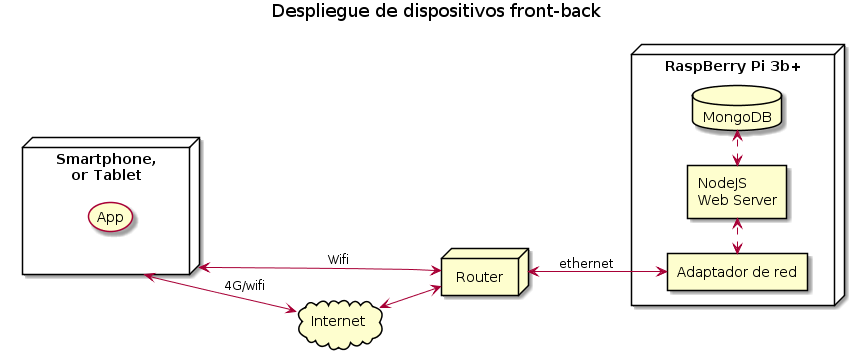
\includegraphics[height=2.5in]{figures/diagrams/physical-devices/front-back.png}
\caption[Despligue de front]{Diagrama de despliegue de smartphone, router y gateway\footnotemark}
\end{figure}



\section{Criterio de selección servicios}
\label{ch:Capitulo4.5}

Al almacenar los datos generados por los nodos en el servidor, en los cuales una medida esta relacionada con un nodo que a su vez esta relacionado con una estancia, plantearse un modelo de \gls{bbdd} relacional es una buena opción. Pero si consideramos que, cada entrada almacenada tendrá una estructura distinta, hace que no sea la opción mas ideal. Por ejemplo, utilizando una \gls{bbdd} SQL se planifica un conjunto de tablas relacionadas entre sí. Es necesaria una tabla que contenga las ubicaciones y se relacione con otra tabla que defina a los nodos. Esto establece una relación 1:N donde múltiples nodos pueden existir para una estancia, pero nunca, un nodo podra estar en varias instancias a la vez simultáneamente. De cada nodo existirá una nueva relación 1:N de medidas. Lo cual deja un esquema semejante al de la figura siguiente:

\begin{figure}[hbt!]
\centering
\label{sqlschema1}
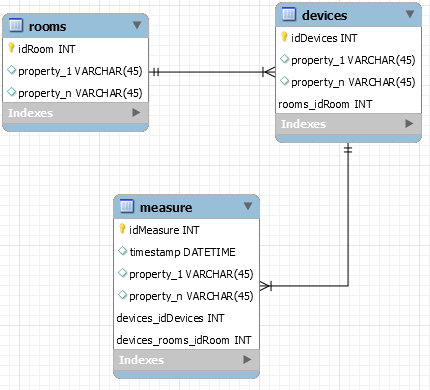
\includegraphics[height=2.5in]{figures/SQLSchemaExample_1.png}
\caption[Primer planteamiento de diseño de BBDD relacional]{Primer planteamiento de diseño de BBDD relacional\footnotemark}
\end{figure}

\vspace{1cm}

Existen algunos problemas graves de diseño de esta idea. En primer lugar, los dispositivos no pueden ser una propiedad de una estancia. Son objetos relacionados, pero no existe una \verb|transitividad dura| entre ellos. Un nodo puede cambiar de estancia en un momento dado, y aun así, seguir existiendo medidas en fechas concretas de ese dispositivo para una habitación en la cual, dicho nodo ya no está relacionado. Otro posible escenario es la desaparición de una estancia (como resultado de fusionar 2 estancias en una al derribar una pared). Para mantener una integridad lógica y persistente a lo largo del tiempo. Toda medida deberá tener un campo que determine en que ubicación fue tomada. No hay transitividad dura entre room y device, lo cual hace que sean independientes entre sí. El siguiente esquema representado en la figura~\ref{sqlschema2} de relación solventa este problema.


\begin{figure}[hbt!]
\centering
\label{sqlschema2}
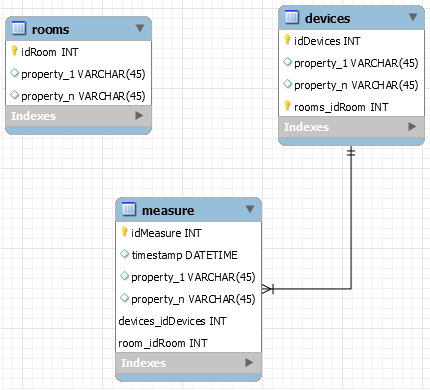
\includegraphics[height=2.5in]{figures/SQLSchemaExample_2.png}
\caption[Segundo planteamiento de diseño de BBDD relacional]{Primer planteamiento de diseño de BBDD relacional\footnotemark}
\end{figure}

\vspace{1cm}

Con esto, aún hay que enfrentar un problema adicional. El número de columnas que definen las propiedades de una tabla. El ejemplo más claro, es la tabla de medidas. Una medida, efectuada por un nodo será definida por su identificador y la fecha en la que se realizó, ahora bien, según la naturaleza del dispositivo, se obtendrán disantos tiempos de medida. Un sensor combinado de temperatura y humedad nos dará dos magnitudes de medición, un sensor de ruido almacenará un valor de decibelios, una luz define su medida por su estado de actividad (encendido o apagado), aunque por otra parte podría indicar el consumo eléctrico, o propiedades adicionales como intensidad de luz, o incluso color (con conjunto de valores RGB). Es cierto que, para un actuador, como lo es un emisor de luz, no realiza medidas como tal, y sus correspondientes estados de actividad podrían ser más adecuados definirlos como propiedades del dispositivo y no como medidas. Podríamos separar las medidas de los estados en tablas distintas, pero igualmente llegaríamos al problema del número de campos necesarios en una tabla. Valor que por otra parte es muy difícil de prever en base a la extensa gama de dispositivos existentes. Esto puede solucionarse de manera sencilla con 2 estrategias.

\begin{enumerate}
  \item Incluir una gran cantidad de columnas en previsión de los distritos tipos de medidas existentes, dejando que las medidas posean un valor nulo para los campos no utilizados en función de la relación de su sensor.

  \item Integración de múltiples opciones de hardware compatibles con la suite domótica.

  \item unificar todos los campos en un único valor de cadena de caracteres que almacene un dato estructurado, como es el caso de los \gls{json}. Esta última opción, sería la más deseable tanto por sencillez de implementación como facilidad de procesamiento.
\end{enumerate}

Lo que dejaría un esquema como el reflejado en la siguiente figura\ref{sqlschema3}.

\begin{figure}[hbt!]
\centering
\label{sqlschema3}
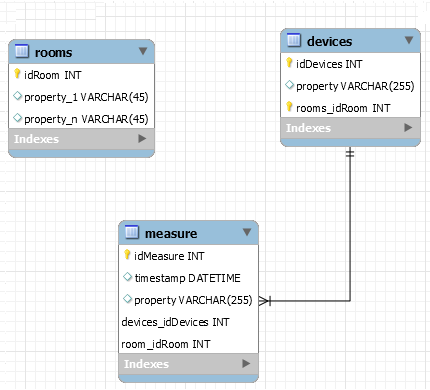
\includegraphics[height=2.5in]{figures/SQLSchemaExample_3.png}
\caption[Tercer planteamiento de diseño de BBDD relacional]{Primer planteamiento de diseño de BBDD relacional\footnotemark}
\end{figure}

\vspace{1cm}

Una preocupación que agrava la perspectiva de usar una \gls{bbdd} relacional es, en este punto del proyecto, su escalabilidad horizontal. Si bien las tablas pueden crecer a un gran número de registros, no se prevé almacenar datos con vistas a largo plazo, la mayoría de los valores almacenados serán efímeros en tiempo de utilidad, almacenarlos responde solo a la necesidad de obtener comparativas en plazos de tiempo relativamente cortos, como horas, días, y posiblemente semanas. Mas allá de este rango estos datos no tienen una utilidad real y pueden ser condensados en medias para utilizarse en resúmenes. Por otro lado, disponer de flexibilidad a la hora de configurar la extensión de propiedades de un objeto de la \gls{bbdd} es uno de los puntos fuertes de una \gls{bbdd} no relacional.


\section{Arquitectura de la aplicación frontend}
\label{ch:Capitulo4.6}

\subsection{Consideraciones previas en el desarrollo de una APP}
\label{c:Capitulo4.6.1}

El desarrollo de la app frontend se ha servido de dos frameworks para salvar ciertos escollos básicos no relacionados con la implementación de la suite domótica. Por un lado, se ha hecho uso del framework Open Source Ionic (en su versión 3), que es un framework Open Source para la construcción de aplicaciones híbridas multiplataforma, que nos permitirá portar la aplicación para cualquier dispositivo móvil Android a través de Cordova, y que además nos permitirá hacer uso de capacidades nativas de los dispositivos móviles (como el módulo de Wifi) gracias a los plugins existentes para ello. Además, Ionic proporciona grandes herramientas en cuanto a la maquetación responsive, lo cual ayuda en la creación de una aplicación móvil sin necesidad de invertir grandes esfuerzos en alcanzar un aspecto, usabilidad y elegancia mínimos y pudiendo redirigir ese esfuerzo a otros terrenos más fructíferos. Ionic está basado en Angular, el otro framework del que se ha hecho uso (en su versión 5) especialmente por su enfoque en una arquitectura basada en componentes que puedan ser reutilizados con mucha facilidad a lo largo de toda la aplicación. Las versiones modernas de Angular hacen uso de TypeScript para la programación de su lógica de negocio, lo que permite una mayor limpieza de código, mejores herramientas de tipado estricto y redunda en mayor escalabilidad. Angular se programa en TypeScript para la lógica de negocio, SASS para los estilos css y HTML para la maquetación.


\subsection{Estructura básica}
\label{ch:Capitulo4.6.2}

A grandes rasgos, la aplicación frontend está estructurada en:
\begin{enumerate}
 \item Componentes, por lo general tendremos casi tantos como trozos o segmentos en los que se quiera desestructurar una vista (los conoceremos como \textit{component}; serán útiles para aislar los diferentes comportamientos que se puede requerir en cada vista, y un mismo componente puede ser replicado infinitamente a lo largo de la aplicación cada vez con unos parámetros diferentes.
 \item Módulos de vistas, generalmente uno por cada vista de la aplicación (lo que conoceremos como \textit{view} o \textit{template}); se encargarán de cargar la información que requiere la vista y de transformar las interacciones del usuario con la vista en flujos lógicos que generalmente pasan por (o acaban en) otros módulos.
 \item Centros de gestión y manipulación de datos, generalmente uno por cada estructura de datos existente (lo que conoceremos como \textit{store}); su cometido será proporcionar métodos a otros módulos o vistas para obtención y/o manipulación de su tipo de datos, siendo la store la responsable última de obtenerlos, manipularlos o almacenarlos por cualquier medio existente.
 \item Servicios que ejercerán de cómodas APIs contra APIs externas o contra \gls{bbdd} locales del dispositivo (los que conoceremos como \textit{api provider/service} en el primer caso y \textit{database service} en el segundo), generalmente uno de cada por cada estructura de datos existente; son responsables de lanzar las llamadas a dichos servicios con los parámetros adecuados (bien seas APIs REST remotas o \gls{bbdd} locales) y controlar sus respuestas.
 \item Servicios, que implementan utilidades y herramientas a lo largo de toda la aplicación de forma independiente, tanto que, técnicamente, podrían formar parte de cualquier otra aplicación (los que conoceremos como \textit{service}); son responsables de aportar utilidades puntuales con la suficiente abstracción como para que el "usuario" de dicho servicio no conozca su funcionamiento en detalle, sino más bien, le resulte sencillo, conveniente y cómodo acudir a sus métodos.
\end{enumerate}

\vspace{0.5cm}

Con el fin de comprender el esquema utilizado, mencionaremos los tipos de estructura existentes, aun cuando detallaremos su flujo más adelante: tendremos los dispositivos, que serán conocidos como \textit{things} (siendo posiblemente lo más adecuado debido a su famosa acepción en el \gls{iot}); las habitaciones, que mencionaremos aquí y allá como \textit{rooms}; los usuarios, que conoceremos como \textit{users}; las placas, que mencionaremos como \textit{boards}; y los datos de aplicación generales, a los que nos referiremos como \textit{application data}. Se observará que, en todos los casos, nos conviene referirlos en su traducción al inglés por facilidad a la hora de seguir el hilo del flujo en el código.

\subsection{Patrón del flujo de datos}
\label{ch:Capitulo4.6.3}

En pro de aplicar una arquitectura que intenta aplicar los principios de separación de responsabilidades y capas de abstracción, a continuación explicamos los patrones que sigue la estructura del proyecto frontend.

\begin{figure}[hbt!]
\centering
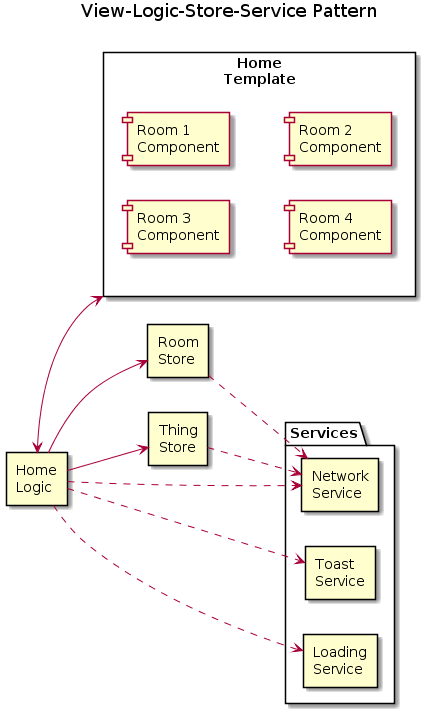
\includegraphics[height=5in]{figures/diagrams/front/architecture/view-logic-store-service-pattern.png}
\caption[view-logic-store-service-pattern]{View-Logic-Store-Service Pattern\footnotemark}
\label{fig:front-view-store}
\end{figure}

\vspace{0.5cm}

Por lo general, todas las vistas presentan, bajo un formato u otro, una serie de datos. El template será por tanto responsable de adaptar y mostrar estos datos como se requiera; pero primero deben obtenerlos, para lo cual delegarán en la store. A partir del momento en que se pide estos datos a la store, se crea una conveniente capa de abstracción que es útil en dos sentidos principales: por un lado, la vista no debe preocuparse del origen de dónde obtener esos datos, esto será responsabilidad de la store, lo cual hace más limpio el código del template, que debe preocuparse estrictamente de atender a los requisitos y cambios de la vista; por otro, la misma lógica que deba implementar la store para ofrecer estos datos a una vista, podrá ser reaprovechada para ofrecérselo a otra. 

\vspace{1cm}

En el ejemplo de la Figura \ref{fig:front-view-store}, podemos observar como el template de la vista \textit{Home} debe mostrar una lista de todas las habitaciones existentes. Una vez el template ha adquirido este array de rooms a partir de la room store, deberemos mostrar un componente room por cada room en esa lista. Sin embargo, la longitud de esta lista no es conocida de antemano, y puede cambiar en cualquier momento. Por tanto, la implementación debe ajustarse a este dinamismo. Angular nos permite, mediante su directiva \textit{ngFor}, generar tantos elementos como existan en un array de la lógica asociada al template, y además pueden ser elementos de cualquier tipo, luego esto nos sirve para crear una lista de componentes room, siendo posible instanciar cada uno con la información específica de cada elemento del array.

\vspace{1cm}

Observaremos que tanto la lógica asociada a una vista como las stores (así como otros services) hacen uso de los services. Estos services ofrecen, de forma autónoma e independiente, ciertas utilidades, como por ejemplo el LoadingService, que ofrece un spinner de carga con un mensaje de feedback para el usuario de que un proceso está cargando. El encargado de poseer y ejecutar la lógica que crea y muestra el spinner será el LoadingService; sin embargo, quien manda la orden inicial será siempre quien invoca al servicio, pues es quien conoce el estado actual de la vista: si los datos han sido pedidos y está a la espera de recibirlos, pedirá mostrar el spinner; si finalmente se recibe confirmación de que la vista ya tiene disponibles los datos, se ordenará ocultar el spinner. 

\vspace{1cm}

\begin{figure}[hbt!]
\centering
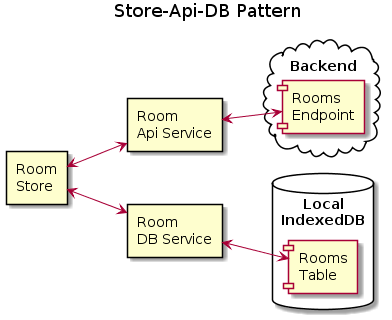
\includegraphics[height=2.5in]{figures/diagrams/front/architecture/store-api-db-pattern.png}
\caption[store-api-db-pattern]{Store-API-DB Pattern\footnotemark}
\label{fig:front-store-api-db}
\end{figure}

Respecto a la obtención de los datos, utilizamos el patrón asociado a la Figura \ref{fig:front-store-api-db}. La store mantiene el rol más importante del flujo del frontend. Observaremos que, cada vez que un componente, vista o módulo desea interactuar con un ejemplar del tipo que regenta la store, por ejemplo, cada vez que un módulo desee obtener la información de una determinada habitación o desee cambiar uno de sus parámetros, pedirá esa información o ese cambio a la room store. Será en ese momento cuando la store decidirá de dónde obtener la información del objeto room, o a qué servicio externo (API o \gls{bbdd} local) hacerle la petición de cambio. Así, veremos que la store hará las veces de distribuidor de la información de su tipo.

\vspace{1cm}

En este punto, con el fin de ejercer la separación de responsabilidades, hemos creado un módulo api provider (específicamente orientado para el mismo tipo de datos que la store) que permite a la store interactuar con la API remota de su mismo tipo; así, cuando la room store quiere obtener del backend la última lista real de rooms disponibles, hará uso del método \verb|getAllRooms| del room provider; de la misma forma, cuando bajo petición del usuario, quiera crear una nueva room, debe hacerse esta petición al servidor a través del método \verb|createRoom| del room provider. Cada una de estas peticiones http a la API remota puede requerir de unas características particulares, como puedan ser su tipo CRUD, los headers http requeridos, la url particular de la petición y la estructura del cuerpo; y al delegar en el api provider, se evitar exponer a la store detalles intrínsecos a la petición http, que debería resultar comportarse como una caja negra de cara a la store, ya que no requiere ese nivel de detalle para su cometido de distribuir la información. 
Es necesario apuntar que todos los api service que hemos creado (en general un por cada tipo de dato importante, o quizás más precisamente, uno por cada endpoint de entrada existente en la API remota), heredan de la clase ApiGenericProvider, la que implementa los métodos CRUD con los que interactuar con la API remota. En la Figura \ref{fig:api-services} se expone el diagrama de clases para todas las APIs creadas.

\begin{figure}[hbt!]
\centering
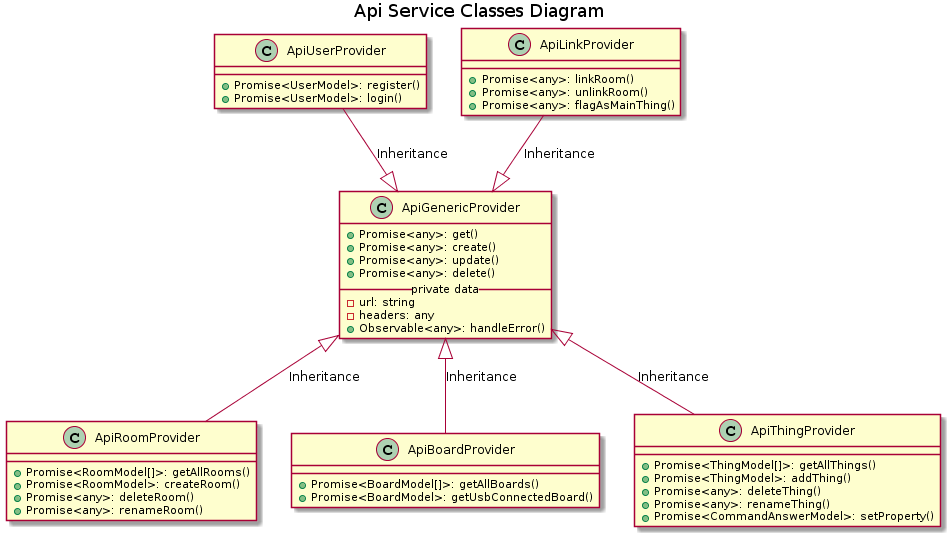
\includegraphics[height=4in]{figures/diagrams/front/architecture/api-services.png}
\caption[api-services]{API Providers Class Diagram\footnotemark}
\label{fig:api-services}
\end{figure}

\vspace{1cm}

De la misma forma y con el mismo objetivo que para el api provider, se crea un módulo database service (específicamente orientado para el mismo tipo de datos que la store), que permite a la store interactuar con la \gls{bbdd} local para almacenar, recuperar o borrar cualquier entrada de ese tipo. En este proyecto, de entre las posibilidades existentes, hacemos uso de la base de datos IndexedDB, propia del motor web del dispositivo. Es una base de datos No-SQL que está orientada al almacenamiento de entradas de gran tamaño, y no bloquea la entrada-salida del hilo principal, de forma que es ideal para almacenar objetos JSON, que puedan tener estructuras y tamaños variables. En particular, cada database service se creará de forma que ataque específicamente a una única tabla, nombrada con el mismo tipo de datos, con el objetivo de reforzar la mantenibilidad del código y la separación de responsabilidades. Así, de nuevo, la store se permite desconocer si sus datos deben tener una estructura, codificación o formato en particular dependiendo de las características de la \gls{bbdd}: delega esa responsabilidad en el database service, el cual debe garantizar que los datos sean devueltos a la store en el mismo formato en que fueron entregados en primera instancia. 
Los módulos database service, a diferencia de los api providers, no heredan de un mismo módulo, pero queda pendiente como una mejora posible puesto que cada uno puede ser creado con una configuración particular (como ya ocurre) y, con la excepción de algunos métodos, se puede refactorizar todos aquellos que sean comunes en una clase padre. En la Figura \ref{fig:database-service} se expone la clase que sigue RoomDatabaseService, muy similar a la que siguen el resto de database services con sus configuraciones propias. Hemos adjuntado un diagrama de cada uno de ellos en el apartado \ref{ch:Capitulo4.6.4}.


\begin{figure}[hbt!]
\centering
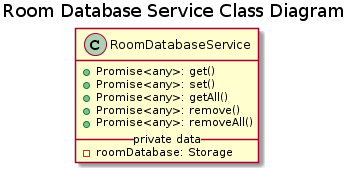
\includegraphics[height=1.5in]{figures/diagrams/front/architecture/database-service.png}
\caption[app-data]{Room Database Service Class Diagram\footnotemark}
\label{fig:database-service}
\end{figure}

\subsection{Inicialización de la aplicación frontend}
\label{ch:Capitulo4.6.4}

Cuando la aplicación Android se inicia, tras las inicializaciones propias del framework de Ionic y Angular, se ejecuta la lógica correspondiente a \verb|app.module.ts|, el módulo base que se encarga de importar todo los módulos que se hemos implementado para nuestra aplicación antes de ejecutarlos por primera vez. El sistema de carga de módulos con \textit{lazy loading} de Angular permite ejecutar algunos de ellos antes que el resto si, por necesidades de la aplicación, es condición necesaria que se procese antes que los demás. En nuestro caso, hacemos uso de esta herramienta para lanzar el método \verb|initializeEndpoint| del módulo \verb|core.module.ts|, que redirige al \verb|initializeApiEndpoints| de \verb|application-data.store.ts| y permite extraer de la \gls{bbdd} local las IPs local y remota para poder disponer de ellas en la inicialización de los servicios de interacción con las APIs remotas.
\vspace{0.5cm}
Tras esto, se crea el \verb|app.component.ts| que representa al componente base sobre el cual se lanza todo el sistema de páginas para cada vista y los módulos contenidos en todos ellos. En su constructor, se llama al método \verb|initializeApplication| del \verb|application.service.ts| (explicado más adelante) para que, en cuanto éste esté listo, oculte el \textit{splash} inicial (en la aplicación Android) y podamos ver la página por defecto, la página de \textit{Login}.
\vspace{0.5cm}
Describimos a continuación la inicialización de servicios y stores de la aplicación frontend, llevada a cabo en el \verb|application.service.ts|. Los pasos siguientes ejecutan una serie de procesos asíncronos, pero la separación en pasos describe cómo cada proceso espera a que el anterior acabe, fin que logramos gracias a las promesas del \verb|ECMASCRIPT 6|. Si alguno de los pasos finalizara erróneamente, el proceso de inicialización no continua y la aplicación no avanzará, debiendo así ser reiniciada.
\begin{enumerate}
\item Se ejecuta el método \verb|_onCordovaEnvironment| que comprueba si la plataforma que se está corriendo es una plataforma construida por Cordova, que nos permite ejecutar esta aplicación web en el dispositivo móvil Android (así como en otros), por lo que esta condición es necesaria para el correcto funcionamiento de toda la lógica del proyecto.
\item Se ejecuta el método \verb|_initializeServices| que inicializa todos aquellos Services que utilizamos y deben ser inicializados. Primero lo hace con el \verb|network.service.ts|, y cuando éste está listo, inicializa el \verb|offline-reminder.service.ts| y el \verb|navigation.service.ts|. Se explica cada uno en detalle en su apartado en la siguiente sección.
\item A continuación, es necesario preparar todos los módulos que necesitan hacer cambios si el estado de autenticación del usuario cambia, con el fin de permitir (o no) a la aplicación mostrar al usuario rutas autorizadas o no (si el token de sesión expiró, se debe impedir que el usuario pueda acceder a información o comandos fuera de su permiso hasta que vuelva a conseguir un token válido). Así, se llama al método \verb|listenAuthenticationStatus| de todas las stores, así como al \verb|subscribeAuthenticationStatus| del \verb|navigation.service.ts| el cual enrutará a la vista de Login si detecta que se ha perdido la autenticación del usuario, o enrutará a la vista de Home si detecta que ha conseguido un token válido.
\item Por último, se lanza el método \verb|initializeUser| para iniciar sesión en la aplicación con un usuario previamente almacenado, si existe y tiene un token que no haya expirado todavía.
\end{enumerate}

\subsection{Diagramas de clases de las Stores, Models y Services}
\label{ch:Capitulo4.6.5}

\begin{figure}[hbt!]
\centering
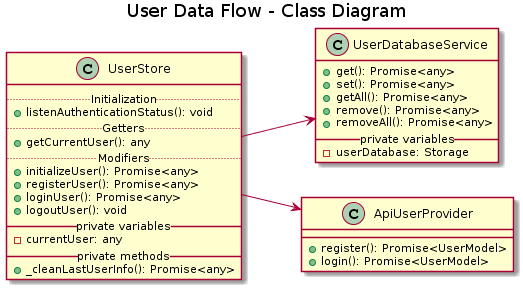
\includegraphics[height=2.5in]{figures/diagrams/front/data-flow/user.png}
\caption[user]{User Data Class Diagram\footnotemark}
\end{figure}

La user store gestiona todo lo relacionado con el login del usuario, es por ello que tiene una fuerte cooperación con el AuthService. Durante la inicialización de la aplicación, se establece una suscripción a cambios de usuarios autenticados en el AuthService con el método público \verb|listenAuthenticationStatus|.

\vspace{0.5cm}

Nuestro proyecto implementa JWT de Auth0, para la autenticación de usuario mediante tokens, lo cual agiliza el login sin necesidad de que el usuario deba introducir de nuevo sus credenciales, y puede ser parametrizado desde el backend. Durante la inicialización de la aplicación, se lanza el método \verb|initializeUser|, el cual busca en la userDB (local del dispositivo) la existencia de un JWT válido. Si lo encuentra, entonces puede pasarle el token al AuthService, el cual lo descifrará y extraerá el usuario autenticado, y establecerá el estado de autenticado del AuthService a verdadero. De esta manera, se la suscripción del \verb|listenAuthenticationStatus| da lugar a pedirle a AuthService el usuario autenticado y se establece como el usuario actual. Si no, se lanza el método privado \verb|_cleanLastUserInfo| para borrar cualquier información remanente en la aplicación móvil relativa al último usuario logado, acudiendo a todas las demás stores para que se encarguen de borrar de sus \gls{bbdd} locales la información pertinente de la que son responsables.

\vspace{1cm}

Además de esto, la user store posee los métodos \verb|loginUser| y \verb|registerUser| que gestionan todo lo relacionado con los intentos de registrar y de iniciar sesión contra la API remota de user mediante el userProvider. Si logra logarse correctamente, el endpoint de login devuelve un token válido que la app almacena en la userDB y que utiliza para el propósito explicado anteriormente, además de pasar al AuthService este token válido para autenticar al usuario.

\begin{figure}[hbt!]
\centering
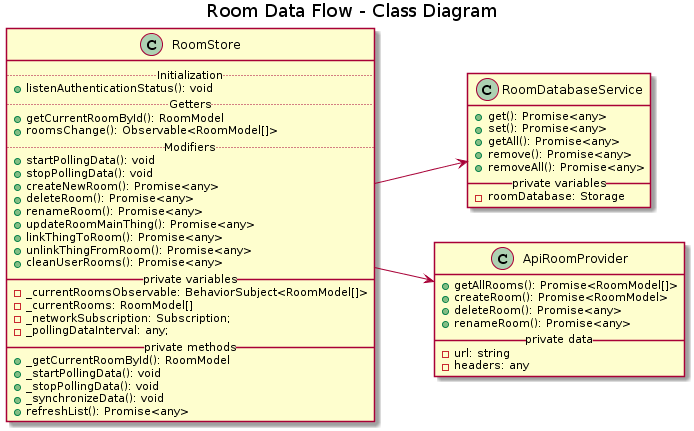
\includegraphics[height=3.5in]{figures/diagrams/front/data-flow/room.png}
\caption[room]{Room Data Class Diagram\footnotemark}
\end{figure}

\vspace{1cm}

La room store gestiona todo lo relacionado con la lista de rooms disponibles. Durante la inicialización de la aplicación, se establece una suscripción a cambios de usuarios autenticados en el AuthService con el método público \verb|listenAuthenticationStatus|; y alinea esta suscripción con otra al estado de la red con el NetworkService, de forma que, si hay conexión a la red y además el usuario está autenticado, se llama al método privado \verb|_startPollingData| (y de lo contrario, llama al \verb|_stopPollingData|).

\vspace{1cm}

\verb|_startPollingData| se encarga de llamar a intervalos de tiempo regulares de 5 segundos al método privado \verb|_synchronizeData|, el cual hace uso del roomProvider para obtener la lista de todas las rooms. Cada vez que interactuemos con la API remota (con cualquiera de sus métodos, y aplicable al resto de stores), ejecutaremos un flujo que consiste en recibir la información, guardarla en la roomDB y llamar al método \verb|refreshList|, que se encarga de extraer el valor actual de esa lista de la roomDB y actualizar tanto el array privado \verb|_currentRooms| como el observable \verb|_currentRoomsObservable| con el nuevo valor.

\vspace{1cm}

Este último paso es crucial para el flujo de datos en la aplicación y representa uno de los patrones reconocidos más útiles de los que hacemos uso en la aplicación frontend: el patrón Observer/Subscribe. La librería RXJs nos ofrece este elemento tan importante, mediante el cual cualquier flujo de la aplicación que desee hacer uso de la lista de rooms, se suscribe al observable \verb|_currentRoomsObservable| mediante el método \verb|roomsChange| de la room store. Cada vez que la room store actualice este observable, el cambio será automáticamente notificado a todos los suscriptores de dicho observable.

\vspace{1cm}

La room store también ofrece los métodos \verb|createNewRoom|, \verb|deleteRoom|, \verb|renameRoom|, \verb|updateRoomMainThing|, \verb|linkThingToRoom| y \verb|unlinkThingFromRoom|. Los tres primeros son autodescriptivos, interactuan con la API y siguen el mismo flujo de actualización descrito anteriormente aunque adaptado a cada caso. Los tres últimos son llamados desde la thing store como parte de unos procesos encadenados, en los cuales se requiere que se cambie información específica de alguna room en particular, pero esta vez sólo de forma local (en el dispositivo), ya que la petición al backend realizada desde la thing store ya desencadena otros flujos secundarios en el backend que actualizan la información de la room implicada. Se garantiza la alineación de datos ya que el flujo está diseñado como si de una transacción se tratara: el backend siempre tiene la información verídica, y si ocurriera algún fallo en el flujo (sea en backend o en frontend), se rechaza el flujo para evitar datos incorrectos, que en cualquier caso serán actualizados con la siguiente petición \verb|_synchronizeData|. 
La room store también expone el método \verb|cleanUserRooms|, accedido y usado desde la user store para el borrado de datos de rooms.

\begin{figure}[hbt!]
\centering
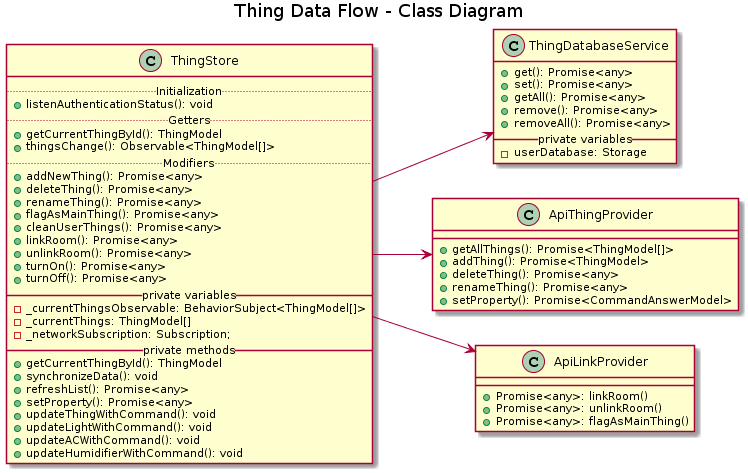
\includegraphics[height=4in]{figures/diagrams/front/data-flow/thing.png}
\caption[thing]{Thing Data Class Diagram\footnotemark}
\end{figure}

La thing store gestiona todo lo relacionado con la lista de things disponibles. Tanto la suscripción al AuthService, y al NetworkService, como el sistema de petición periódica y recuperación de datos, así como la exposición del observable a posibles suscriptores, es idéntico al de room store pero evidentemente aplicado a la lista de things, por lo cual no entraremos en detalle de nuevo.

\vspace{1cm}

La thing store también ofrece los métodos \verb|addNewThing|, \verb|deleteThing|, \verb|renameThing|, \verb|flagAsMainThing|, \verb|linkRoom| y \verb|unlinkRoom|, que interactuan con la API en sus métodos homónimos y siguen el mismo flujo de actualización descrito anteriormente aunque adaptado a cada caso. Los tres últimos 

La thing store también expone el método \verb|cleanUserThings|, accedido y usado desde la user store para el borrado de datos de things.


\begin{figure}[hbt!]
\centering
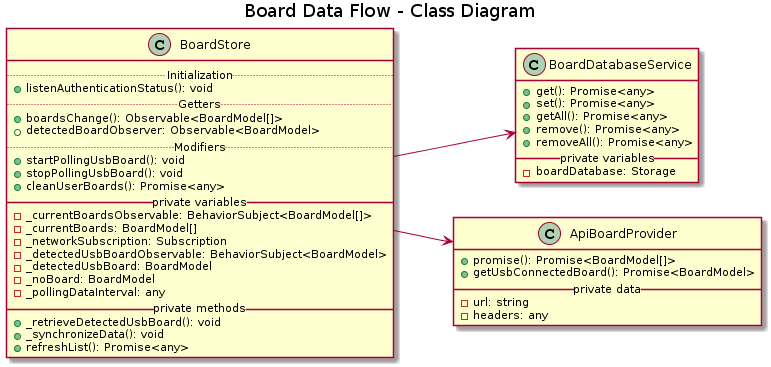
\includegraphics[height=3.5in]{figures/diagrams/front/data-flow/board.png}
\caption[thing]{Board Data Class Diagram\footnotemark}
\end{figure}

La board store gestiona todo lo relacionado con las boards disponibles. La implementación actual, para el objetivo del proyecto, no requiere almacenar una lista de boards disponibles como ocurre con las stores de rooms o things; sin embargo, dispone de todo el flujo y todos sus métodos, al igual que con las otras stores, lo cual puede resultar útil para futuras ampliaciones del proyecto. El aspecto más importante de esta store es su flujo de detección de una placa conectada al puerto USB de la Raspberry Pi, preguntando periódicamente al backend, con el fin de comunicárselo a los módulos interesados en ejecutar alguna acción dependiendo de esto. Este flujo es explicado en contexto en el caso de uso \ref{ch:Capitulo5.2.4}.

\begin{figure}[hbt!]
\centering
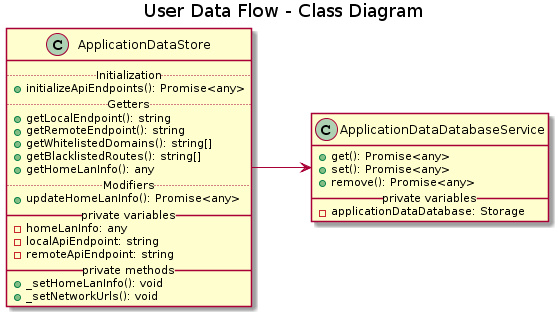
\includegraphics[height=3in]{figures/diagrams/front/data-flow/app-data.png}
\caption[app-data]{Application Data Class Diagram\footnotemark}
\end{figure}

La application data store gestiona toda la información general que la aplicación requiere almacenar y utilizar y que puede varia con las acciones del usuario; principalmente se encargará de almacenar y modificar las URLs locales y remotas a las cuales la aplicación debe apuntar, según las circunstancias.
Si el usuario se encuentra en la misma red local que la Raspberry Pi, mediante una acción del menú \textit{Settings} podrá detectar la red actual y recordarla (IP local y SSID), mediante el método de la store \verb|updateHomeLanInfo|, para así comunicarse por Wifi con el nodo principal, pudiendo prescindir de una conexión de Internet y la respectiva cobertura. Si por el contrario, se encuentra usando una red de datos (o una red Wifi desconocida, en la que no se encuentra la Raspberry Pi), utilizará la URL que apunta a la IP externa en la cual encontrar a la Raspberry Pi. Para setear las URLs a usar por los servicios de API remota, la store lanza el método \verb|_setNetworkUrls| que cambia la info utilizada en el \verb|network.service.ts|, el punto que utilizan dichas APIs. sus métodos \verb|getLocalEndpoint| y \verb|getRemoteEndpoint|.
De la misma forma, es la store encargada de ofrecerle al módulo JWT las rutas permitidas y las prohibida, mediante los métodos \verb|getWhitelistedDomains| y \verb|getBlacklistedRoutes| respectivamente.

\begin{figure}[hbt!]
\centering
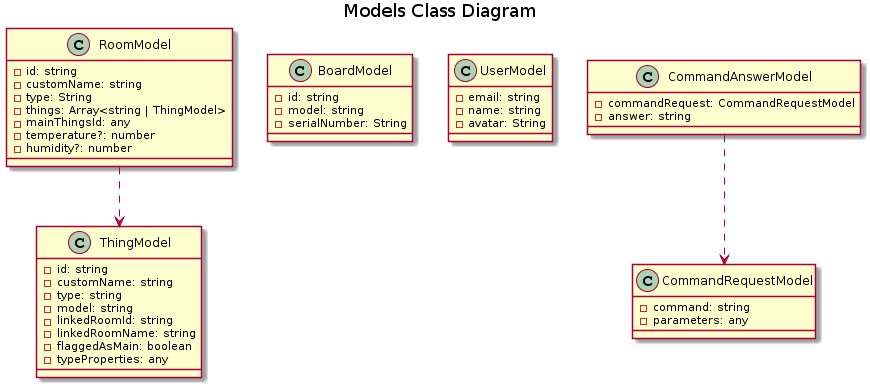
\includegraphics[height=3in]{figures/diagrams/front/architecture/models.png}
\caption[models]{Models Classes Diagram\footnotemark}
\end{figure}

Los diagramas de clase responden a modelos para cada tipo de datos que sean claros y concisos, permitiendo toda la operatividad requerida para los casos de uso existentes.
\begin{enumerate}

\item Para la clase \verb|RoomModel|, se requiere un \verb|id| como identificador único de la room, un  \verb|customName| como "identificador humano" para el usuario, el \verb|type| para categorizar el tipo de estancia (útil a la hora de presentar las habitaciones y discernir mediante una imagen y un símbolo el tipo de habitación a simple vista), un campo \verb|things| para almacenar la lista de things asociadas a dicha room (es de tipo variable ya que en ciertos momentos de su flujo, serán simplemente identificadores, y en otros, serán las \verb|ThingModel| como objetos completos), un objeto \verb|mainThingsId| donde señalar la thing principal de cada tipo para dicha room y un campo \verb|sensorMeasures| donde almacenar los cálculos generales extraidos de sus sensores asociados a la room.

\item Para la clase \verb|ThingModel|, se requiere un \verb|id| como identificador único de la thing, un  \verb|customName| como "identificador humano" para el usuario, el \verb|type| para categorizar el tipo de thing (si es de tipo luz, de tipo sensor, etc.), un campo \verb|model| para distinguir el modelo específico que rige el comportamiento de dicha thing, un campo \verb|linkedRoomId| y otro \verb|linkedRoomName| para marcar la room a la que está asociada la thing, un booleano \verb|flaggedAsMain| para mostrarlo y distinguirlo del resto de things del mismo tipo asociadas a la misma room, y un \verb|typeProperties| donde van todas las características, valores y detalles de dicha thing.

\item Para la clase \verb|UserModel|, sólo es requerido su \verb|email| como campo único, siendo su \verb|nombre| y \verb|avatar| opcionales para mostrar el perfil del usuario logado.

\item Para la clase \verb|CommandRequestModel|, usamos un campo \verb|command| que marca el comando a ejecutar sobre una determinada thing y el campo \verb|parameters| marca los parámetros opcionales que requiere dicho comando.

\item Para la clase \verb|CommandAnswerModel|, el campo \verb|commandRequest| es del tipo \verb|CommandRequestModel| y contiene el objeto comando para el cual este objeto es la respuesta al comando, así como un campo \verb|answer| opcional que pueda añadir algún detalle o información de respuesta.

\end{enumerate}

\begin{figure}[hbt!]
\centering
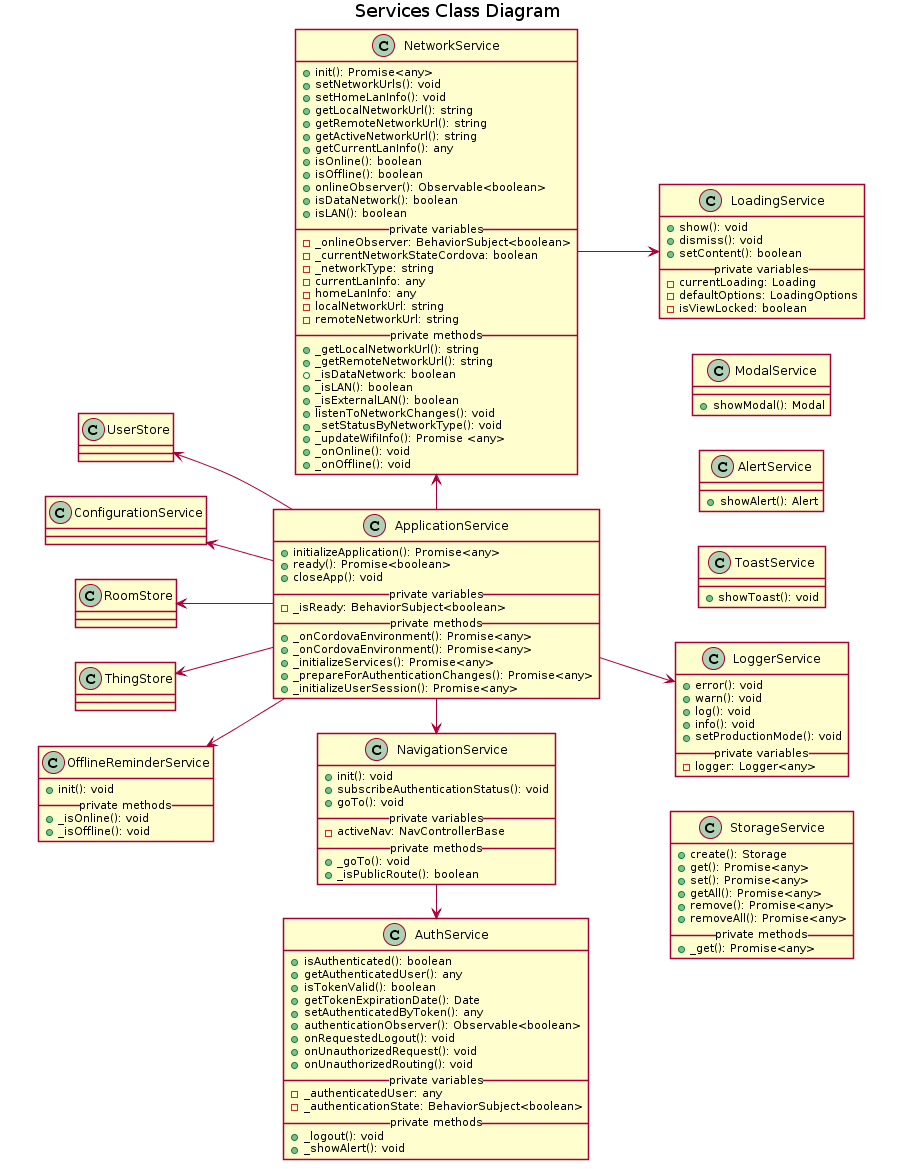
\includegraphics[height=8.2in]{figures/diagrams/front/architecture/services.png}
\caption[services]{Services Class Diagram\footnotemark}
\end{figure}

[EXPLICAR AQUÍ LOS SERVICES]

\section{Arquitectura del servidor de NodeJS}
\label{ch:Capitulo4.7}

\subsection{Consideraciones previas}
\label{ch:Capitulo4.7.1}

El desarrollo de la aplicación backend ha seguido la línea del stack MEAN, esto es, MongoDB, ExpressJS, Angular (éste sólo en el frontend) y NodeJS. Los beneficios de seguir dicho stack son sencillamente los de sus frameworks y herramientas: MongoDB aporta los beneficios de una \gls{bbdd} no relacional, enormemente alineado con las características del proyecto, según el cual podríamos almacenar grandes cantidades de datos con diferentes estructuras JSON bajo la misma lista de documentos sin perder velocidad de acceso o escritura; ExpressJS nos permite elaborar una API REST completa salvando los principales escollos que NodeJS podría presentarnos para tal fin, pues sus herramientas base para el tratamiento de peticiones http se presentan intrincadas y poco intuitivas; y NodeJS se beneficia de infinitas librerías de sencillo uso, constantemente probadas y actualizadas por su amplia comunidad, proveyéndonos en este caso de muchas utilidades que nos ayudan a evitar desarrollos difíciles e innecesarios no intrínsecos a una suite domótica (como es nuestro fin) y cuyos beneficios enumeraremos más adelante.

\subsection{Estructura básica}
\label{ch:Capitulo4.7.2}

A grandes rasgos, la aplicación backend está estructurada en:
\begin{enumerate}
 \item Enrutadores, por lo general tendremos uno por cada nombre en nuestra API REST (los conoceremos como \textit{routers}); gracias a ExpressJS, permiten encaminar cada petición http recibida en el servidor según su tipo CRUD (GET, POST, PUT o DELETE) y la estructura de la URL asociada, para ser atendida por el método específico que debe procesar dicha petición.
 \item Controladores, por lo general tendremos uno por cada nombre en nuestra API REST (los conoceremos como \textit{controllers}); encuadran un contexto en el que se crea, manipula, sirve, guarda y destruye elementos de la estructura de datos asociada, además de exponer una serie de métodos, generalmente uno por cada posible entrada de la API para el nombre de dicha API asociado a la estructura de datos en uso.
 \item Modelos, de los que tendremos uno por cada estructura de datos existente (los conoceremos como \textit{models}); definirán la estructura JSON que debe seguir un objeto para ser incluido en una collección de MongoDB, y que utilizaremos para generar y reconocer objetos de dicho tipo de estructura de datos y poder mejorar la interacción con la \gls{bbdd} de MongoDB.
 \item Servicios, que al igual que en el proyecto frotend, ejercerán de cómodas APIs contra diferentes servicios, como pueda ser la \gls{bbdd} de MongoDB, el protocolo \gls{mqtt} y otros módulos de utilidades (los conoceremos como \textit{providers} o \textit{services}); por lo general, podrían ser prácticamente independientes y ser copiados tal cual a cualquier otro proyecto (a falta de ligeras adaptaciones que en lineas generales facilitan su explotación en cada caso) y proporcionan una capa de abstracción adicional que delimita la responsabilidad del módulo que hace uso de dicho servicio y reduce su complejidad de código.
 \item Módulos de soporte, por lo general tendremos tantos como sean necesarios, y cada uno se dedica exclusivamente a un tipo de estructura de datos (los conoceremos como helpers); ofrecen sus métodos tanto a su controller asociado como a otros controllers, de forma desacoplada con el fin de aligerar la carga de código del controller asociado.
 \item Módulos intermediarios, que aportan utilidades adicionales a la hora de procesar peticiones http (los conoceremos como \textit{middlewares}); gracias a ExpressJS, permitirán enriquecer el tratamiento de dichas peticiones para establecer filtros adicionales o transformaciones de los datos de la petición.
 \item Archivos de configuración y de constantes, que permitirán aislar adecuadamente el uso de constantes útiles a lo largo de toda la aplicación, de una forma centralizada, independiente y de fácil acceso y modificación.
\end{enumerate}

Con el fin de comprender el esquema utilizado y establecer una alineación con el frontend, la nomenclatura utilizada para cada tipo de datos será la misma que en el proyecto cliente.

\subsection{Flujo de enrutado de las peticiones HTTP}
\label{ch:Capitulo4.7.3}

\begin{figure}[hbt!]
\centering
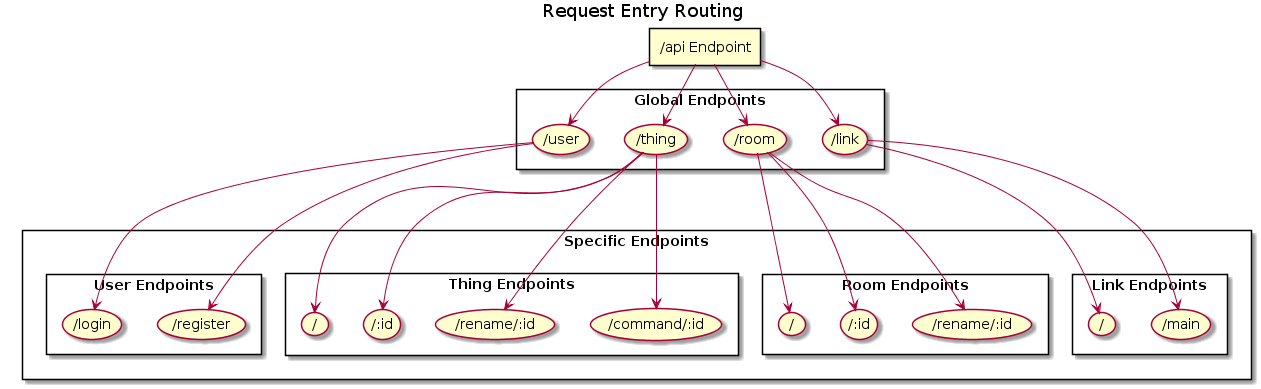
\includegraphics[height=2.5in]{figures/diagrams/back/router-flow/api-entry.png}
\caption[api-entry]{Base API Entry Schema\footnotemark}
\label{fig:back-api-entry}
\end{figure}

Como hemos explicado anteriormente, ExpressJS es utilizado para el enrutado de toda petición HTTP que alcance la aplicación backend. Durante la inicialización del servidor, mediante el método \verb|listen| en el \verb|server.js| se utiliza el objeto \verb|app| expuesto en el \verb|src/app.js| (un objeto generado por el framework ExpressJS) para generar un servidor que atenderá todas las peticiones HTTP en el puerto que se le configure, en este caso, se ha designado el puerto 3000.
\vspace{0.5cm}
Posteriormente, se lanza el setup del enrutador con el método \verb|setupRouting| del módulo \verb|router.js|, el cual se encarga de importar todos los routers existentes y vincularlos a cada uno de los endpoints que serán atendidos mediante el método \verb|use| del objeto \verb|app|. Así, suponiendo que se recibe una petición http con la ruta \verb|/api/thing|, ésta será redirigida al router \verb|thingRouter| mediante el método y sus parámetros \verb|use(ROUTER_CONFIG.EP_GLOBAL.THINGS, thingRouter)|. El primer nivel de encaminamiento de las peticiones es tal que el mostrado en la Figura \ref{fig:back-api-entry}.
\vspace{0.5cm}
Una vez la petición ha sido encaminada a un router en particular, entramos en el segundo nivel de encaminamiento. En este punto, el router se encarga de importar el controller específico para su tipo de datos y de encaminar cada endpoint a la función final de un controller que atenderá a dicha petición. ExpressJS nos permite registrar dicha función a ejecutar para unas características particulares de petición, de forma que con unos sencillos métodos, podremos asociar dicho método dependiendo del tipo CRUD de la petición atendida y de las características de su URL. Así, suponiendo que nuestro \verb|thing.router.js| atiende una petición PUT en la url \verb|/api/thing/rename/:id|, mediante el método \verb|put| podremos encaminar dicha petición a ser atendida por el método \verb|renameThing| del \verb|thing.controller.js|. Este segundo nivel de encaminamiento de las peticiones es tal que el mostrado en cada una de las figuras siguientes, brevemente descrito para cada endpoint.

\begin{figure}[hbt!]
\centering
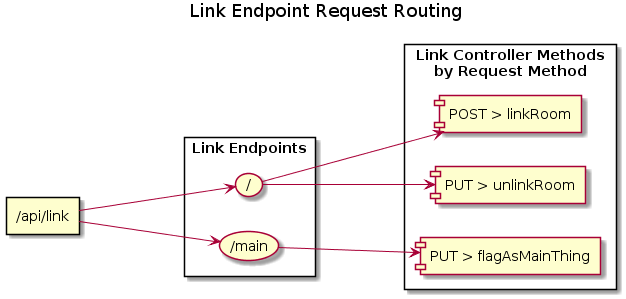
\includegraphics[height=2.5in]{figures/diagrams/back/router-flow/link-endpoints.png}
\caption[link-endpoints]{Link API Schema\footnotemark}
\end{figure}

Para el endpoint \verb|/api/link|, se asocian 3 entradas atendidas por el \verb|link.router.js|:
\begin{enumerate}
\item En la ruta \verb|/api/link/|, las peticiones POST serán atendidas por el método \verb|linkRoom|.
\item En la ruta \verb|/api/link/|, las peticiones PUT serán atendidas por el método \verb|unlinkRoom|.
\item En la ruta \verb|/api/link/main|, las peticiones PUT serán atendidas por el método \verb|flagAsMainThing|.
\end{enumerate}

\begin{figure}[hbt!]
\centering
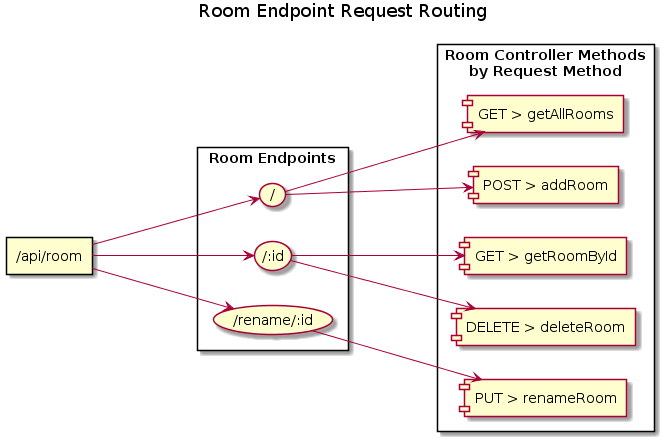
\includegraphics[height=2.5in]{figures/diagrams/back/router-flow/room-endpoints.png}
\caption[room-endpoints]{Room API Schema\footnotemark}
\end{figure}

Para el endpoint \verb|/api/room|, se asocian 5 entradas atendidas por el \verb|room.router.js|:
\begin{enumerate}
\item En la ruta \verb|/api/room/|, las peticiones GET serán atendidas por el método \verb|getAllRooms|.
\item En la ruta \verb|/api/room/|, las peticiones POST serán atendidas por el método \verb|addRoom|.
\item En la ruta \verb|/api/room/:id|, las peticiones GET serán atendidas por el método \verb|getRoomById|.
\item En la ruta \verb|/api/room/:id|, las peticiones DELETE serán atendidas por el método \verb|deleteRoom|.
\item En la ruta \verb|/api/room/rename/:id|, las peticiones PUT serán atendidas por el método \verb|renameRoom|.
\end{enumerate}

\begin{figure}[hbt!]
\centering
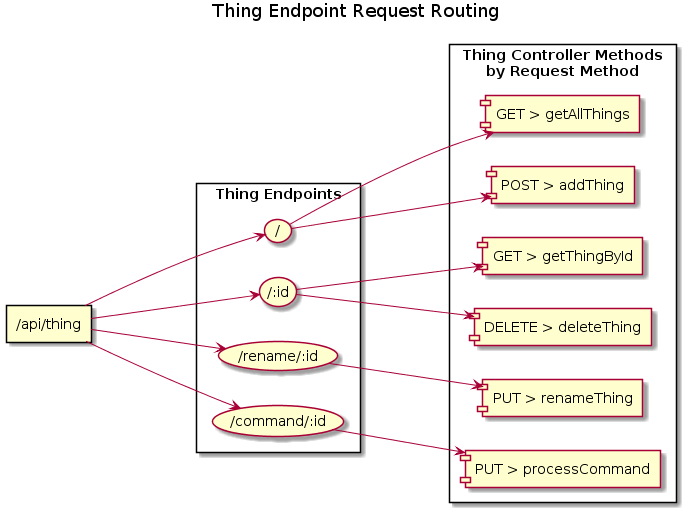
\includegraphics[height=2.5in]{figures/diagrams/back/router-flow/thing-endpoints.png}
\caption[thing-endpoints]{Thing API Schema\footnotemark}
\end{figure}

Para el endpoint \verb|/api/thing|, se asocian 6 entradas atendidas por el \verb|thing.router.js|:
\begin{enumerate}
\item En la ruta \verb|/api/thing/|, las peticiones GET serán atendidas por el método \verb|getAllThings|.
\item En la ruta \verb|/api/thing/|, las peticiones POST serán atendidas por el método \verb|addThing|.
\item En la ruta \verb|/api/thing/:id|, las peticiones GET serán atendidas por el método \verb|getThingById|.
\item En la ruta \verb|/api/thing/:id|, las peticiones DELETE serán atendidas por el método \verb|deleteThing|.
\item En la ruta \verb|/api/thing/rename/:id|, las peticiones PUT serán atendidas por el método \verb|renameThing|.
\item En la ruta \verb|/api/thing/command/:id|, las peticiones PUT serán atendidas por el método \verb|processCommand|.
\end{enumerate}

\begin{figure}[hbt!]
\centering
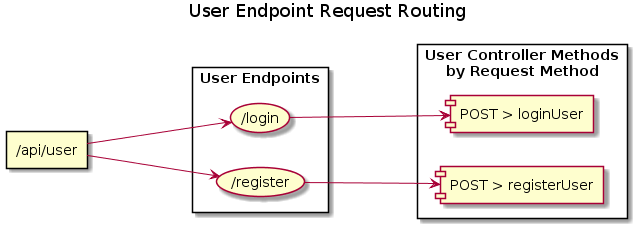
\includegraphics[height=2.5in]{figures/diagrams/back/router-flow/user-endpoints.png}
\caption[user-endpoints]{User API Schema\footnotemark}
\end{figure}

Para el endpoint \verb|/api/user|, se asocian 2 entradas atendidas por el \verb|user.router.js|:
\begin{enumerate}
\item En la ruta \verb|/api/link/login|, las peticiones POST serán atendidas por el método \verb|loginUser|.
\item En la ruta \verb|/api/link/register|, las peticiones POST serán atendidas por el método \verb|registerUser|.
\end{enumerate}

\begin{figure}[hbt!]
\centering
\includegraphics[height=2.5in]{figures/diagrams/back/router-flow/board-endpoints.png}
\caption[board-endpoints]{Board API Schema\footnotemark}
\end{figure}

Para el endpoint \verb|/api/board|, se asocian 2 entradas atendidas por el \verb|board.router.js|:
\begin{enumerate}
\item En la ruta \verb|/api/board/|, las peticiones GET serán atendidas por el método \verb|getAllBoards|.
\item En la ruta \verb|/api/board/detect|, las peticiones GET serán atendidas por el método \verb|getUSBConnectedBoard|.
\end{enumerate}

[HABLAR AQUÍ DE MIDDLEWARES]
[passport.middleware.js]


Toda petición http que no sea encaminada a un método mediante esta metodología será automáticamente rechazada. Esto permite controlar severamente los caminos por los cuales se ejecutará una lógica en base a una petición http, y por ende constituye una medida de seguridad adicional por el principio básico de conocer y controlar todas las posibles entradas al servidor con un flujo único y específico para cada una de ellas, para minimizar brechas de seguridad.

\subsection{Diagramas de clases de los Controllers, Helpers y Models}
\label{makereference4.7.4}

[HABLAR AQUÍ DE CONTROLLERS]

El \verb|core.controller.js| se encarga de lanzar aquellos procesos que deben estar listos tras la inicialización base del servidor NodeJS. Una vez el servidor ha conectado su cliente de Mongo a la instancia de MongoDB, está listo para interactuar con toda la información almacenada anteriormente en la \gls{bbdd}, y el proceso de \verb|app.js| se encarga de lanzar el método \verb|setupCoreMonitors| del coreController. Este método lanza dos de sus métodos internos, por un lado \verb|_launchStoredSubscriptions| y posteriormente \verb|_releaseDaemons|, finalizando así la preparación inicial del servidor.

\vspace{0.5cm}

El método \verb|_launchStoredSubscriptions| se encarga de extraer de la base de datos la lista actual de things y, mediante el método \verb|generateSubscriptionData| del \verb|thing.helper.js|, genera una lista de objetos con información de suscripciones MQTT para cada thing que esté operativa (es decir, vinculadas a una habitación). Tras esto, transfiere dicha lista al \verb|mqtt.service.js| para que inicialice su servicio mediante su método \verb|initializeClient|.
Posteriormente, el método \verb|_releaseDaemons| se encarga de lanzar, a intervalos regulares de 5 segundos, a los \textit{daemons} (denominados así por sus características de funcionamiento) para que paulatinamente realicen sus operaciones regulares, mediante el método \verb|roomDaemon| del \verb|room.controller.js| y el método \verb|thingDaemon| del \verb|thing.controller.js|. Serán explicados en detalle en sus respectivos apartados.

\vspace{1cm}

El \verb|room.controller.js| se encarga de, por un lado, correr el \verb|roomDaemon| mencionado previamente, y por otro, exponer sus métodos vinculados a la API REST.
Por un lado, el \verb|roomDaemon| (recordemos que este método es invocado de forma regular cada 5 segundos de operación del servidor) se encarga de calcular la media de las medidas de los sensores DHT11 y MQ135 que haya en cada habitación, y almacenar dicho cálculo en el campo sensorMeasures de cada habitación. Esta operación se lleva a cabo siguiendo los siguientes pasos:
\begin{enumerate}
    \item Extrae las rooms disponibles en la colección de Rooms de MongoDB, y para cada habitación, lleva a cabo los pasos siguientes pasos.
    \item Obtiene la lista de things vinculada a dicha habitación mediante el método \verb|getThingsByRoom| del \verb|thing.controller.js|, y discrimina en dos listas diferentes los things que corresponden a sensores DHT11 y los que corresponden a sensores MQ135.
    \item Con la ayuda del \verb|thing.helper.js|, los métodos \verb|getDHT11AvgInfo| y \verb|getMQ135AvgInfo| calculan la información media útil de dichos sensores.
    \item Actualiza la room analizada en la MongoDB con esta información almacenada en su campo \verb|sensorMeasures|.
\end{enumerate}

\vspace{0.5cm}

El método \verb|getAllRooms| extrae de la MongoDB la lista de rooms almacenadas, y si la operación ha tenido éxito, resuelve la petición http con un código 200 y la lista de rooms en el body de la respuesta; de lo contrario, devuelve un código 500 y un mensaje de error.
El método \verb|getRoomById| extrae de la MongoDB la room con el campo id igual al parámetro id en la URL de la petición http, y si la operación ha tenido éxito, resuelve la petición http con un código 200 y la room recuperada en el body de la respuesta; de lo contrario, devuelve un código 500 y un mensaje de error.
El método \verb|addRoom| crea un objeto del tipo Room con un id pseudoaleatorio y los campos customName y type coincidentes con los valores del body de la petición http. A continuación, procede a salvar este objeto en la colección de Rooms de la MongoDB, y si la operación ha tenido éxito, resuelve la petición http con un código 200 y la nueva room creada en el body de la respuesta; de lo contrario, devuelve un código 500 y un mensaje de error.
El método \verb|deleteRoom| elimina de la MongoDB la room con el campo id igual al parámetro id en la URL de la petición http, y si la operación ha tenido éxito, resuelve la petición http con un código 200 y un mensaje de éxito; de lo contrario, devuelve un código 500 y un mensaje de error.
El método \verb|renameRoom| modifica en la MongoDB la room con el campo id igual al parámetro id en la URL de la petición http, sustituyendo el valor de su campo customName por el proporcionado en la petición http, y si la operación ha tenido éxito, resuelve la petición http con un código 200 y un mensaje de éxito; de lo contrario, devuelve un código 500 y un mensaje de error.

\vspace{1cm}

El \verb|thing.controller.js| se encarga principalmente de, por un lado, correr el \verb|thingDaemon| mencionado previamente, y por otro, exponer sus métodos vinculados a la API REST.
En este caso, por el momento, el método \verb|thingDaemon| no contiene operaciones requeridas pero se mantiene por su potencial utilidad en futuras versiones del proyecto.

\vspace{0.5cm}

El método \verb|getAllThings| extrae de la MongoDB la lista de things almacenadas, y si la operación ha tenido éxito, resuelve la petición http con un código 200 y la lista de things en el body de la respuesta; de lo contrario, devuelve un código 500 y un mensaje de error.
El método \verb|getThingsByRoom| realiza la misma operación que el \verb|getAllThings|, pero sólo extrae de la MongoDB la lista de things almacenadas vinculadas a una room en particular, y devuelve el valor. Este método no atiende a la API REST, sólo responde como utilidad del controller en sí.
El método \verb|getThingById| extrae de la MongoDB la thing con el campo id igual al parámetro id en la URL de la petición http, y si la operación ha tenido éxito, resuelve la petición http con un código 200 y la thing recuperada en el body de la respuesta; de lo contrario, devuelve un código 500 y un mensaje de error.
El método \verb|addThing| crea un objeto del tipo Thing con un id pseudoaleatorio y los campos customName, type y model coincidentes con los valores del body de la petición http. Además, en su campo typeProperties, almacena una estructura con datos por defecto dependiendo del type y model especificados (gracias al método \verb|getModelStructure| del \verb|thing.helper.js|). A continuación, procede a salvar este objeto en la colección de Things de la MongoDB, y si la operación ha tenido éxito, resuelve la petición http con un código 200 y la nueva thing creada en el body de la respuesta; de lo contrario, devuelve un código 500 y un mensaje de error.
El método \verb|deleteThing| elimina de la MongoDB la thing con el campo id igual al parámetro id en la URL de la petición http, y si la operación ha tenido éxito, resuelve la petición http con un código 200 y un mensaje de éxito; de lo contrario, devuelve un código 500 y un mensaje de error.
El método \verb|renameThing| modifica en la MongoDB la thing con el campo id igual al parámetro id en la URL de la petición http, sustituyendo el valor de su campo customName por el proporcionado en la petición http, y si la operación ha tenido éxito, resuelve la petición http con un código 200 y un mensaje de éxito; de lo contrario, devuelve un código 500 y un mensaje de error.
El método \verb|processCommand| se encarga de procesar un comando específico para la thing con id igual al parámetro id de la petición http. Primero, obtiene la thing coincidente almacenada en la MongoDB; segundo, obtiene una instancia del controlador específico para dicha thing según su tipo; y por último, ejecuta el método \verb|processRequest| de dicha instancia con los datos de la thing y el comando de la petición. El resultado de este último método expone un flujo de éxito y otro de fracaso. Si la operación ha tenido éxito, resuelve la petición http con un código 200 y un objeto JSON confirmando el éxito del comando solicitado; de lo contrario, devuelve un código 500 y un mensaje de error.

\vspace{1cm}

El \verb|link.controller.js| se encarga de exponer sus métodos vinculados a la API REST.

\vspace{0.5cm}

El método \verb|linkRoom| se encarga de vincular una thing a una room y de ordenar todo lo necesario para el funcionamiento de dicha thing de forma independiente. Con el fin de evitar repeticiones, se refiere a la sección \ref{ch:Capitulo5.3.2} para la explicación de este método, pues el contexto proporcionado en dicha sección ofrece una mejor visión del cometido de este método.
El método \verb|unlinkRoom| realiza una operación inversa al \verb|linkRoom|. Así, se encarga de eliminar las referencias mutuas entre la thing de la petición y su room asociada en sus respectivas colecciones Rooms y Things; y cuando esto ha ocurrido con éxito, se encarga de llamar al método \verb|removeSubscription| del \verb|mqtt.service.js| para eliminar tanto la suscripción de \textit{idThing/status} como la de \textit{idThing/answer}; y si la operación ha tenido éxito, resuelve la petición http con un código 200 y un mensaje de éxito; de lo contrario, devuelve un código 500 y un mensaje de error.
El método \verb|flagAsMainThing| se encarga de marcar a la thing de la petición http como principal de su tipo en su room vinculada. Por un lado, actualiza el campo \verb|flaggedAsMain| de la thing (previamente actualiza el mismo campo la anterior thing del mismo tipo marcada como principal antes que ésta, si existe, sustituyéndola así); por otro lado, actualiza en la MongoDB el campo \verb|mainThingsId| de la room asociada en la propiedad pertinente según el tipo de la thing; y si la operación ha tenido éxito, resuelve la petición http con un código 200 y un mensaje de éxito; de lo contrario, devuelve un código 500 y un mensaje de error.

\vspace{1cm}

El \verb|board.controller.js| se encarga de exponer sus métodos vinculados a la API REST.

\vspace{0.5cm}

El método \verb|getAllBoards| extrae de la MongoDB la lista de boards almacenadas, y si la operación ha tenido éxito, resuelve la petición http con un código 200 y la lista de boards en el body de la respuesta; de lo contrario, devuelve un código 500 y un mensaje de error.
El método \verb|getUSBConnectedBoard| se encarga de devolver la board conectada en ese momento al puerto USB de la Raspberry Pi. Con el fin de evitar repeticiones, se refiere al paso 4 de la sección \ref{ch:Capitulo5.3.4} para la explicación de este método, pues el contexto proporcionado en dicha sección ofrece una mejor visión del cometido de este método.

\vspace{1cm}

El \verb|user.controller.js| se encarga de exponer sus métodos vinculados a la API REST.

\vspace{0.5cm}

El método \verb|registerUser| comprueba en la colección Users de la MongoDB si existe un usuario con el email proporcionado en la petición http. Si ya existe, devuelve un código 500 y un mensaje de error; si no existe, crea un nuevo objeto User con las características email y password del body de la petición y lo almacena en la MongoDB. Si la operación ha tenido éxito, resuelve la petición http con un código 200 y un mensaje de éxito; de lo contrario, devuelve un código 500 y un mensaje de error.
El método \verb|loginUser| comprueba en la colección Users de la MongoDB si existe un usuario con el email proporcionado en la petición http. Mediante el método del esquema User \verb|comparePassword|, procede a devolver si el login ocurre con éxito o no, resolviendo la petición http con un código 200 y un objeto JSON con el email y un token válido (creado por el método privado \verb|_createToken|) o bien devolviendo un código 400 y un mensaje de error.
El método privado \verb|_createToken| hace uso del plugin JWT para crear un token único con el id de usuario y su email, siguiendo la configuración existente en los campos \verb|JWT_SECRET| y \verb|TOKEN_EXPIRE_TIME| del \verb|server.config.js|.

[HABLAR AQUÍ DE LIGHT CONTROLLER]
[HABLAR AQUÍ DE SENSOR CONTROLLER]

[HABLAR AQUÍ DE HELPERS]
[thing.helper.js
  translateCommand,
  getThingControllerInstance,
  generateSubscriptionData,
  getModelStructure,
  getDHT11AvgInfo,
  getMQ135AvgInfo
]

\vspace{1cm}
Los modelos utilizados en el backend se diseñan como modelo para su \gls{bbdd} de MongoDB, y por ello la creación del modelo es mediante los métodos \verb|Schema| y \verb|model| de la librería de npm \verb|mongoose|. Estos modelos, a excepción del User, siguen el mismo esquema que los utilizados en el frontend, lo que refuerza la mantenibilidad de código y permite una comunicación con menos trabas entre cliente y servidor. El modelo Board, va asociado a la colección de MongoDB 'Boards'; el modelo Room, va asociado a la colección de MongoDB 'Rooms'; el modelo Thing, va asociado a la colección de MongoDB 'Things'; y el modelo User, va asociado a la colección de MongoDB 'Users'.
Particularmente, para el modelo User, posee 2 campos, \verb|email| (identificador único, alineado con el frontend), y \verb|password| para almacenar el password del usuario. Además, se definen unos métodos en relación con su cometido de identificación de usuario para inicios de sesión. Se establece un método que es ejecutado justo antes de almacenar objetos de tipo User en la MongoDB (cuando se registra un nuevo usuario), que gracias a la librería de npm \verb|bcryptjs|, permite aplicar \gls{salt} y \gls{hash} sobre el password como medidas adicionales de seguridad. Además, se establece otro método para la comparación de password, en el flujo ejecutado cuando un usuario intenta hacer login. Este método también utiliza la librería de \verb|bcryptjs| para comparar bajo las mismas condiciones de \gls{salt} y \gls{hash}.

\subsection{Diagramas de clases de los Services}
\label{makereference4.7.5}

El servicio \verb|mqtt.service.js| ofrece la capacidad de interactuar de forma sencilla con otros dispositivos mediante el protocolo MQTT, apoyándose en la librería de npm \verb|mqtt|, mediante los métodos que expone, que explicamos a continuación.
\begin{enumerate}
\item El método \verb|initializeClient| permite inicializar un cliente MQTT y conectarlo a un broker mediante una URL. Una vez ha ocurrido, ejecuta el método privado \verb|_loadSubscriptions| con una lista existente de suscripciones necesarias, y lanza el método \verb|_initMessageListener| para iniciar la escucha de mensajes MQTT.
\item El método \verb|stopClient| permite cerrar la conexión con dicho broker MQTT.
\item El método \verb|addSubscription| permite suscribir el cliente a un topic formado por un identificador de thing y un endpoint, y asociar cualquier mensaje recibido en dicho topic a la ejecución de una función referenciada por parámetro.
\item El método \verb|removeSubscription| permite desuscribir el cliente de un topic formado por un identificador de thing y un endpoint y eliminar la vinculación a funciones asociadas en la suscripción.
\item El método \verb|publish| permite publicar un mensaje en un topic formado por un identificador de thing y un endpoint.
\end{enumerate}
Igualmente importante es el flujo de escucha y procesado de mensajes MQTT, mediante los métodos privados \verb|_initMessageListener| y método privado \verb|_processMessage|, que se encargan de procesar cualquier mensaje recibido por MQTT, extraer del topic el identificador de thing y el endpoint y lanzar la función asociada a dicha combinación de suscripción.

[mqtt.service.js
  initializeClient,
  stopClient,
  addSubscription,
  removeSubscription,
  publish
  
  _loadSubscriptions
  _subscribeTopic
  _unsubscribeTopic
  _publishTopic
  _initMessageListener
  _formTopic
  _findSubscriptionIndex
  _processMessage
  ]
  
El servicio \verb|mongo.db.js| tiene la capacidad de iniciar la conexión entre el proyecto y la \gls{bbdd} de MongoDB. El trabajo en bruto de la conexión ocurre gracias a la librería de npm \verb|mongoose|.El servicio en cuestión expone el método \verb|_connect| que hace uso de esta librería para, mediante eventos de conexión, establecer la conexión con unos parámetros dados de dónde se encuentra la MongoDB (URL y las opciones necesarias para la conexión, valores que se extraen de los campos \verb|MONGODB_URL| y \verb|MONGODB_OPTIONS| del archivo de configuración \verb|server.config.js|), así como escuchar posibles errores de la conexión y avisar de cuándo la conexión ha tenido éxito, para poder asegurar que a partir de entonces las operaciones contra la MongoDB ocurran con ciertas garantías.

\vspace{1cm}
 
El servicio \verb|shell.service.js| tiene la capacidad de ejecutar scripts de shell. Este servicio expone el método \verb|compileAndUploadToBoard| para generar, compilar y cargar a una placa todos los scripts que necesite dicha placa para operar una thing conectada a ella en comunicación con el nodo principal. \verb|compileAndUploadToBoard|, para su fin, hace uso del método privado \verb|_execAsync| y detecta cuando el script devuelve por stdout el string "Ended" como señal de finalización. En ese caso, 
Su método privado \verb|_execAsync| hace el trabajo en bruto gracias al uso de la librería de npm \verb|shelljs|, ejecutando el script de shell que recibe por parámetro. Controla las salidas stdout y stderr para ejecutar una función en caso de resultados devueltos por la salida stdout, o ejecutar otra en caso de errores devueltos por la salida stderr.

\vspace{1cm}

El servicio \verb|usb.service.js| es capaz de detectar dispositivos USB conectados al dispositivo sobre el cual corre el proceso de NodeJS.
Este servicio expone el método \verb|initListening| para indicar al servicio que empiece a escuchar los posibles cambios en dispositivos conectados, así como el \verb|stopListening| para indicar al servicio que deje de escuchar dichos cambios. Además, expone el método \verb|getCurrentConnectedUSB| para devolver el dispositivo conectado actualmente. Todo el trabajo en bruto es facilitado por la librería de npm  \verb|usb-detection| que interactua con el sistema operativo para ofrecer esta información.
